\part{决策分析}
多目标决策分析(Multi-Criteria Decision Analysis,MCDA)是依据备择决策方案(Alternatives)的不同特征(属性、准则或目标)构造偏好模型,用以辅助决策、提升决策效率与效果的一门学科。假设备选决策方案集合$\mathcal{A}=\{A_i\}_{i=1}^m$,决策准则集合$\mathcal{C} = \{C_j\}_{j=1}^n$,如下表所示:
\begin{table}[ht]
\caption{MCDM决策矩阵}\label{tbl:decisionmatrix}
\centering
\begin{tabular}{l|llll}
  \hline
   & $C_1$ & $C_2$ & $\cdots$ & $C_n$\\
  \hline
   & $\omega_1$ & $\omega_2$ & $\cdots$ & $\omega_n$\\
  \hline
  $A_1$ & $a_{11}$ & $a_{12}$ & $\cdots$ & $a_{1n}$ \\
  $A_2$ & $a_{21}$ & $a_{22}$ & $\cdots$ & $a_{2n}$ \\
  $\vdots$ & $\vdots$ & $\vdots$ & $\ddots$ & $\vdots$ \\
  $A_m$ & $a_{m1}$ & $a_{m2}$ & $\cdots$ & $a_{mn}$ \\
  \hline
\end{tabular}
\end{table}
表中,第一行是准则集合$\mathcal{C}$,第二行表示准则的权重向量$\omega$,第一列表示备选决策方案集$\mathcal{A}$,$a_{ij}$表示方案$A_i$在准则$C_j$下的表现。

MCDA解决的问题包括:搜索最佳决策方案、对决策方案分类、根据偏好对决策方案排名、描述每个决策方案同时满足所有准则的程度,经典的方法包括数据包络分析方法(Data Envelopment Analysis,DEA)、层次分析法(Analytic Hierarchy Process,AHP)\cite{saaty1977scaling,saaty1980analytic}、
ELETRE\cite{roy1968classement}、PROMETHEE和TOPSIS。

\chapter{数据包络分析}

\ornamento
\section{引言}
效率(绩效)评价在现实生活中是一项常见并且重要的工作。但是,当被评价系统存在多输入和多输出指标时,绩效评价工作则变得非常困难,尤其当输入和输出指标之间存在复杂的甚至是未知关系时,评价工作将更加难以进行。数据包络分析(Data Envelopment Analysis,DEA)作为处理多输入多输出系统评价问题的一种有效的非参数效率评价方法,在组织相对效率评价和组织改进投入产出效率方面越来越受到重视。

DEA方法是由Abraham Charnes、William Cooper和Edwardo Rhodes\cite{charnes1978dea}基于“相对效率”(Relative Efficiency)概念发展而来的,常用于评价多输入-多输出类型决策单元(Decision Making Unit, DMU),如医院、银行、政府部门、生产供应商等企事业单位的生产或服务的相对效率。在数据包络分析框架下,相对效率定义为“加权输出总量与加权输入总量的比值”。

假设有$n$个性质完全相同的生产厂商,都是使用原材料$A$生产出产品$B$,各厂商的生产状况如下表:
\begin{table}[htbp]
\centering
\begin{tabular}{|c|c|c|}
  \hline
  DMU & A & B \\
  \hline
  $1$ & $x_1$ & $y_1$ \\
  $2$ & $x_2$ & $y_2$ \\
  \ldots & \ldots& \ldots \\
  $n$ & $x_n$ & $y_n$ \\
  \hline
\end{tabular}
\end{table}

如果需要评价各个厂商的生产效率,就需要一个标准的定量指标。对于单投入-单产出的生产问题,最简单的评价指标莫过于原材料利用率:单位原材料能够产出的产品数量,那么,对于$\mathrm{DMU}_i$,其原材料利用率$e_i = y_i/x_i$,则原材料利用率越高的厂商可以认定其生产效率越高。

然而,原材料利用率忽略了投入-产出价格因素的影响,皆假设“各个厂商以相同的价格购买原材料,产品的定价也是相同的”。实际上,如果从投入-产出的价值(考虑了价格因素,以金钱作为度量单位)角度出发,评价结果不会有任何变化。

在实际生产过程中,单投入-单产出的生产情形几乎不存在,比较常见的利用多用原材料生产多种产品,即多投入-多产出问题。假设存在$n$个同种类型的决策单元,每个决策单元有$m$个输入量$x_{ik},i=1,\ldots,m$,$s$个输出量$y_{rk},r=1,\ldots,s$。

\begin{table}[htbp]\label{tbl:dmu}\caption{决策单元的输入输出}\vskip 2mm
\centering
\begin{tabular}{|c|c|c|c|c||c|c|c|c|}
  \hline
  DMU & $I_1$ & $I_2$ & \ldots & $I_s$ & $O_1$ & $O_2$ & \ldots & $O_m$\\
  \hline
  $1$ & $x_{11}$ & $x_{12}$ & \ldots & $x_{1s}$ &$y_{11}$ & $y_{12}$ & \ldots & $y_{1m}$\\
  $2$ & $x_{21}$ & $x_{22}$ & \ldots & $x_{2s}$ & $y_{21}$ & $y_{22}$ & \ldots & $y_{2m}$\\
  \ldots & \ldots & \ldots & \ldots & \ldots & \ldots & \ldots & \ldots & \ldots\\
  $n$ & $x_{n1}$ & $x_{n2}$ & \ldots & $x_{ns}$ & $y_{n1}$ & $y_{n2}$ & \ldots & $y_{nm}$\\
  \hline
\end{tabular}
\end{table}
每个DMU使用$s$种原材料$I_1,I_2,\ldots, I_s$生产$m$种产品$O_1,O_2,\ldots,O_m$。

从经济学角度来看,各个决策单元对输入原料的利用率千差万别,要衡量DMU使用原料生产产品(输出)的效率,数据包络分析为任意决策单元$\mathrm{DMU}_k$ 定义如下形式的相对效率指标:
\begin{equation}\label{eq:relativeefficient}
  e_k = \frac{u^T y_k}{w^T x_k}
\end{equation}
其中,$u\in \mathbb{R}^s$表示输入权值向量,$w\in \mathbb{R}^m$表示输出权值向量。此外,假设所有生产厂商的相对效率值均小于1,则经典的CCR模型可以表示成如下形式的线性规划问题:
\begin{equation}\label{eq:fracccr}
\begin{array}{ll}
  \max\limits_{w, u} & \dfrac{u^Ty_k}{w^Tx_k}\\
  \textit{s.t.} &\dfrac{u^Ty_j}{w^Tx_j}\leq 1, j=1,2,\dots,n\\
   & w\geq 0, u\geq 0
\end{array}
\end{equation}

从以上模型可以发现,每个决策单元实际上都是从自身角度出发,倾向于选择于自己最有利的输入- 输出“价格”($w,u$)\cite{kao2005dea}。同时,模型对应的最优权值也反映出目标决策单元$\mathrm{DMU}_k$对输入-输出的某种评价。

由于计算分式规划问题比较复杂,引入Charnes-Cooper变换,
\footnote{令$t=1/w^Tx_k$,$\nu=tw$,$\mu=tu$,则有$u^Ty_k/w^Tx_k=\mu^Ty_k/\nu^Tx_k$,$\nu^Tx_k=tw^Tx_k=1$。}
得到如下形式的线性规划模型:
\begin{equation}\label{eq:ccr}
\begin{array}{lllll}
  \max\limits_{\mu,\nu} & \mu^Ty_k & & \min\limits_{\mu,\nu} & \nu^T x_k\\
  \textit{s.t.} & \mu^Ty_j -\nu^Tx_j \le 0, j=1,2,\dots,n & & \textit{s.t.} & \mu^Ty_j -\nu^Tx_j \le 0, j=1,2,\dots,n \\
   & \nu^Tx_k = 1 & & & \mu^T y_k = 1\\
   & \nu\geq 0, \mu\geq 0 & & & \nu\geq 0, \mu\geq 0
\end{array}
\end{equation}
前者为输入型CCR模型,后者为输出型CCR模型。
\footnote{DEA模型根据目标函数的不同,可以分成两类:投入型(Input-Oriented)和产出型(Output-Oriented)。产出型DEA模型是在给定投入生产要素下最大化生产产出,而投入型是在给定产出水品下最小化投入成本。}

在评价决策单元是否为DEA有效时,需要判断是否存在最优解$\nu^{*},\mu^{*}$,满足
\begin{equation}
  \nu^{*} >0, \mu^{*} >0, \mu^{*T}y_k = 1(\nu^{*T}x_k = 1)
\end{equation}

从计算的角度分析,单纯形法(Simplex Method)就可以有效地求解CCR模型\cite{cooper2011data},由于DMU的个数通常远大于用于决策的特征属性(输入-输出)的数目,使用对偶模型对提升求解性能大有裨益。根据线性规划中的对偶理论(Duality Theory),乘法形式(Multiplier Form)的CCR模型等价对偶形式,也称包络形式(Envelopment Form)如下所示:
\begin{equation}\label{eq:dualccr}
\begin{array}{lllll}
  \textit{min} & \theta & & \textit{max} & \theta\\
  \textit{s.t.} &  \sum\limits_{i = 1}^n \lambda_i x_i \le \theta x_k & & \textit{s.t.} & \sum\limits_{i = 1}^n \lambda_i x_i \le x_k\\
   & \sum\limits_{i = 1}^n \lambda_i y_i \ge y_k & & & \sum\limits_{i = 1}^n \lambda_i y_i \ge \theta y_k\\
   & \lambda_i \ge 0, i = 1, \ldots, n & & & \lambda_i \ge 0, i = 1, \ldots, n
\end{array}
\end{equation}

对输入型CCR包络模型添加松弛变量$S^{-},S^{+}$,转化为下式:
\begin{equation}\label{eq:inputdualccr}
\begin{array}{ll}
  \textit{min} & \theta\\
  \textit{s.t.} & \sum\limits_{i = 1}^n \lambda_i x_i + S^{-} = \theta x_k \\
   & \sum\limits_{i = 1}^n \lambda_i y_i - S^{+} = y_k\\
   & \lambda_i \ge 0, i = 1, \ldots, n\\
   & S^{-} \ge 0, S^{+}\ge 0
\end{array}
\end{equation}

根据线性规划对偶理论中的松紧定理,判断决策单元$\mathrm{DMU_k}$是否DEA有效,需要首先判定模型的最优解$\lambda^{*}, S^{-*},S^{+*},\theta^{*}$是否满足
\begin{equation}
  \theta^{*} = 1, S^{-*} = 0, S^{+*} = 0
\end{equation}

无论是利用\eqref{eq:ccr}还是\eqref{eq:inputdualccr},直接判断DEA有效性都不容易。为此,通过引入非阿基米德无穷小量(non-Archimedean)$\varepsilon >0$的概念\cite{charnes1952optimality,charnes1957management},可以成功地解决计算上和技术上的困难。
\begin{equation}\label{eq:eccr}
\begin{array}{lllll}
  \max\limits_{\mu} & \mu^Ty_k & & \min & \theta - \varepsilon(1^T S^{-} + 1^T S^{+}) \\
  \textit{s.t.} & \mu^Ty_j -\nu^Tx_j\leq 0, j=1,2,\dots,n & & \textit{s.t.} & \sum\limits_{i = 1}^n \lambda_i x_i + S^{-} = \theta x_k\\
   & \nu^Tx_k = 1 & & & \sum\limits_{i = 1}^n \lambda_i y_i - S^{+} = y_k\\
   & \nu\geq \varepsilon & & & \lambda_i \ge 0, i = 1, \ldots, n\\
   & \mu\geq \varepsilon & & & S^{-} \ge 0, S^{+}\ge 0
\end{array}
\end{equation}

\section{两阶段方法}%Two-Stage Method
魏权龄在\cite{wei2004dea}给出一个引理:考虑线性规划问题
\begin{equation}
\begin{array}{ll}
  \textit{min} & c^Tx \\
  \textit{s.t.} & Ax = b \\
  & x \ge 0
\end{array}
\end{equation}
若其最优解集合为$\mathbb{E}$,则存在$\bar{\varepsilon} >0$,对于任意的$\varepsilon\in(0,\bar{\varepsilon})$,线性规划问题
\begin{equation}
\begin{array}{ll}
  \textit{min} & c^Tx - \varepsilon d^Tx \\
  \textit{s.t.} & Ax = b \\
  & x \ge 0
\end{array}
\end{equation}
的最优解也是下面线性规划问题的最优解:
\begin{equation}
\begin{array}{ll}
  \textit{max} & d^Tx \\
  \textit{s.t.} & x \in \mathbb{E}
\end{array}
\end{equation}

对于含有非阿基米德无穷小量的对偶CCR模型:
\begin{equation}\label{eq:dualeccr}
\begin{array}{ll}
  \textit{min} & \theta - \varepsilon(1^T S^{-} + 1^T S^{+}) \\
  \textit{s.t.} & \sum\limits_{i = 1}^n \lambda_i x_i + S^{-} = \theta x_k\\
   & \sum\limits_{i = 1}^n \lambda_i y_i - S^{+} = y_k\\
   & \lambda_i \ge 0, i = 1, \ldots, n\\
   & S^{-} \ge 0, S^{+}\ge 0
\end{array}
\end{equation}
可以使用2-阶段法(阶段I与阶段II)求解:
\begin{enumerate}[(I)]
  \item 求解对偶规划
\begin{equation}
\begin{array}{ll}
  \textit{min} & \theta\\
  \textit{s.t.} & \sum\limits_{i = 1}^n \lambda_i x_i + S^{-} = \theta x_k \\
   & \sum\limits_{i = 1}^n \lambda_i y_i - S^{+} = y_k\\
   & \lambda_i \ge 0, i = 1, \ldots, n\\
   & S^{-} \ge 0, S^{+}\ge 0
\end{array}
\end{equation}
    的最优解$\theta^{*}$。如果$\theta^{*} < 1$,则$\mathrm{DMU_k}$不为DEA弱有效;若$\theta^{*} = 1$,则转到阶段II(将最优值$\theta^{*} = 1$带入上述模型中得到其最优解集合)。
  \item 求解下面问题的最优解$\lambda^{*}, S^{-*},S^{+*}$:
\begin{equation}
\begin{array}{ll}
  \textit{max} & 1^T S^{-} + 1^T S^{+} \\
  \textit{s.t.} & \sum\limits_{i = 1}^n \lambda_i x_i + S^{-} = x_k\\
   & \sum\limits_{i = 1}^n \lambda_i y_i - S^{+} = y_k\\
   & \lambda_i \ge 0, i = 1, \ldots, n\\
   & S^{-} \ge 0, S^{+}\ge 0
\end{array}
\end{equation}
如果$1^T S^{-*} + 1^T S^{+*} \ne 0$,则$\mathrm{DMU_k}$弱DEA有效;否则$\mathrm{DMU_k}$DEA有效。
\end{enumerate}

对于$n$个决策单元组成的评价系统,假设参考集为
\begin{equation}
  \hat{T} = \{(x_i, y_i) | i = 1,\ldots, n\}
\end{equation}
形如下面的生产可能集
\begin{equation}
  \mathrm{T_{CCR}} = \{(x,y) | \sum\limits_{i = 1}^n \lambda_i x_i \le x, \sum\limits_{i = 1}^n \lambda_i y_i \ge y, \lambda_i \ge 0, i = 1,\ldots, n\}
\end{equation}
与CCR模型相对应。判断决策单元是否DEA有效,本质上是检验决策单元是否落在生产可能集的生产前沿面上。

假设$\lambda^{*}, S^{-*},S^{+*}, \theta^{*}$是通过$2-$阶段法求解不含有非阿基米德无穷小量的CCR原始模型与对偶模型的最优解,令
\begin{equation}
  \begin{array}{lll}
    \hat{x}_k & = & \theta^{*} x_k - S^{-*} \\
    \hat{y}_k & = & y_k + S^{+*}
  \end{array}
\end{equation}
称$(\hat{x}_k, \hat{y}_k)$是$\mathrm{DMU_k}$在生产可能集$ T_{CCR}$的生产前沿面上的“投影”,根据“投影定理”\cite{wei2004dea},它们是DEA有效的。

DEA能够计算分配效率(Allocate Efficiency,AE)和技术效率(Technical Efficiency,TE),后者分为规模效率(Scale Efficiency, SE)和纯技术效率(Pure Technical Efficiency,PTE),隐含着很强的经济学背景,其中,技术效率与规模效率分别是生产函数和生产函数的规模收益不变性质的推广\cite{wei2004dea}。

\section{DEA变体模型}
1984年,Banker等人\cite{banker1984some}提出一种新的模型——BCC模型,使用凸约束(Convexity Constraint)度量决策单元的技术效率。在凸约束中,可以确保复合决策单元与被评测单元大小相当。BCC模型估计的相对效率值不小于对应CCR模型计算的相对效率分值。BCC与CCR模型不同,后者是基于规模收益不变(Constant Return to Scales,CRS)的假设,而BCC则适用于规模收益可变(Variable Return to Scales,VRS)的场景。
\begin{equation}\label{eq:inputbcc}
  \begin{array}{lllll}
    \textit{max} & \mu^T y_k - u_k & & \textit{min} & \theta\\
    \textit{s.t.} & \mu^T y_i - \nu^T x_i  - u_k \le 0, i = 1,\ldots, n & & \textit{s.t.} & \sum\limits_{i=1}^n \lambda_i x_i \le \theta x_k\\
    & \nu^T x_k = 1 & & & \sum\limits_{i=1}^n \lambda_i y_i \ge y_k\\
    & \nu \ge 0,\mu \ge 0 & & & \sum\limits_{i=1}^n \lambda_i = 1,\lambda_i \ge 0, i = 1,\ldots, n\\
  \end{array}
\end{equation}
此为输入型BCC模型,而输出型BCC模型如下所示:
\begin{equation}\label{eq:outputbcc}
  \begin{array}{lllll}
    \textit{min} & \nu^T x_k + u_k & & \textit{max} & \theta\\
    \textit{s.t.} & \nu^T x_i - \mu^T y_i  + u_k \ge 0, i = 1,\ldots, n & & \textit{s.t.} & \sum\limits_{i=1}^n \lambda_i y_i \ge \theta y_k\\
    & \mu^T y_k = 1 & & & \sum\limits_{i=1}^n \lambda_i x_i \le x_k\\
    & \nu \ge 0,\mu \ge 0 & & & \sum\limits_{i=1}^n \lambda_i = 1,\lambda_i \ge 0, i = 1,\ldots, n\\
  \end{array}
\end{equation}

1985年,F\"{a}re和Grosskopf\cite{fare1985nonparametric}在使用非参数的费用方法研究规模收益时,使用的DEA模型称为FG模型,其基本假设是规模收益递减:
\begin{equation}\label{eq:fg}
  \begin{array}{lllll}
    \textit{max} & \mu^T y_k - u_k & & \textit{min} & \theta\\
    \textit{s.t.} & \mu^T y_i - \nu^T x_i  - u_k \le 0, i = 1,\ldots, n & & \textit{s.t.} & \sum\limits_{i=1}^n \lambda_i x_i \le \theta x_k\\
    & \nu^T x_k = 1 & & & \sum\limits_{i=1}^n \lambda_i y_i \ge y_k\\
    & \nu \ge 0,\mu \ge 0, u_k \ge 0 & & & \sum\limits_{i=1}^n \lambda_i \le 1,\lambda_i \ge 0, i = 1,\ldots, n\\
  \end{array}
\end{equation}

1990年,Seiford与Thrall\cite{seiford1990recent}提出了基于规模收益递增假设下的ST模型:
\begin{equation}\label{eq:st}
  \begin{array}{lllll}
    \textit{max} & \mu^T y_k - u_k & & \textit{min} & \theta\\
    \textit{s.t.} & \mu^T y_i - \nu^T x_i  - u_k \le 0, i = 1,\ldots, n & & \textit{s.t.} & \sum\limits_{i=1}^n \lambda_i x_i \le \theta x_k\\
    & \nu^T x_k = 1 & & & \sum\limits_{i=1}^n \lambda_i y_i \ge y_k\\
    & \nu \ge 0,\mu \ge 0, u_k \le 0 & & & \sum\limits_{i=1}^n \lambda_i \ge 1,\lambda_i \ge 0, i = 1,\ldots, n\\
  \end{array}
\end{equation}

1985年,Charnes等人\cite{charnes1985foundations}认为CCR 模型中关于生产函数凸性的假设在某些条件下是不合理的,将目标规划首次应用到DEA方法,推出了一种新的效率评价模型——加法模型(Additive Model)(亦称“$\mathrm{C^2GS^2}$模型”)。加法模型基于规模收益可变假设,最大化被评估决策单元与有效前沿面(或包络面)的$\ell_1$ 距离。
\begin{equation}\label{eq:c2gs2-l1}
  \begin{array}{ll}
    \textit{max} & ||(x_k, y_k) - (\sum\limits_{i=1}^n \lambda_i x_i,\sum\limits_{i=1}^n \lambda_i y_i)||_1\\
    \textit{s.t.} & x_k \ge \sum\limits_{i=1}^n \lambda_i x_i \\
    & y_k \le \sum\limits_{i=1}^n \lambda_i y_i\\
    & \sum\limits_{i=1}^n \lambda_i = 1\\
    & \lambda_i \ge 0, i =1,\ldots, n
  \end{array}
\end{equation}
由于
\begin{equation}
  \begin{array}{lll}
    & ||(x_k, y_k) - (\sum\limits_{i=1}^n \lambda_i x_i,\sum\limits_{i=1}^n \lambda_i y_i)||_1 \\
    = &  |x_{k1} - \sum\limits_{i=1}^n \lambda_i x_{i1}| + \cdots + |x_{km} - \sum\limits_{i=1}^n \lambda_i x_{im}| + \cdots + |y_{k1} - \sum\limits_{i=1}^n \lambda_i y_{i1}| + \cdots + |y_{k1} - \sum\limits_{i=1}^n \lambda_i y_{is}|\\
    = & (x_{k1} - \sum\limits_{i=1}^n \lambda_i x_{i1}) + \cdots  + (x_{km} - \sum\limits_{i=1}^n \lambda_i x_{im}) + \cdots + (\sum\limits_{i=1}^n \lambda_i y_{i1} - y_{k1}) + \cdots + (\sum\limits_{i=1}^n \lambda_i y_{is} - y_{ks})\\
    = & 1^T S^{-} + 1^T S^{+}
  \end{array}
\end{equation}
从而,可以得到下面等价的加法模型:
\begin{equation}\label{eq:c2gs2}
  \begin{array}{ll}
    \textit{max} & 1^T S^{+}_k + 1^T S^{-}_k\\
    \textit{s.t.} & S^{+}_k = \sum\limits_{i=1}^n \lambda_i y_i - y_k \\
    & S^{-}_k = x_k - \sum\limits_{i=1}^n \lambda_i x_i\\
    & \sum\limits_{i=1}^n \lambda_i = 1\\
    & S^{+}_k \ge 0, S^{-}_k  \ge 0,\lambda_i \ge 0, i =1,\ldots, n
  \end{array}
\end{equation}

原始的DEA模型对权重无任何限制,允许被评估决策单元选择对于自身最有利的权重,得出的结果明显不符合实际,因此,人们一直重视对权重的研究。1986年,Charnes等人\cite{charnes1989cone}通过调整锥比率以反映决策者的偏好或者意愿,给出一个含有偏好的$\mathrm{C^2WH}$模型。

\subsection{一般性DEA模型}
为了分析DEA模型的一般性质,避免无谓的重复工作,研究人员开始构建综合的数据包络分析模型。1988年,Charnes等人\cite{charnes1988compositive}给出了第一个综合的DEA 模型$\mathrm{C^2WY}$,包含CCR模型,加法模型和$\mathrm{C^2WH}$等模型,遗憾的是$\mathrm{C^2WY}$模型不能直接进行编程实现。根据
\cite{yu1996generalized}构造的一般性DEA 模型,可以统一CCR、BCC、FG与ST 模型为下面形式的输入型综合DEA模型:
\begin{equation}\label{eq:uniteddea}
  \begin{array}{lllll}
    \textit{max} & \mu^T y_k - \delta_1 u_k & & \textit{min} & \theta\\
    \textit{s.t.} & \nu^T x_i - \mu^T y_i + \delta_1 u_k \ge 0, i = 1,\ldots, n & & \textit{s.t.} & \sum\limits_{i=1}^n \lambda_i x_i \le \theta x_k\\
    & \nu^T x_k = 1 & & & \sum\limits_{i=1}^n \lambda_i y_i \ge y_k\\
    & \nu \ge 0,\mu \ge 0 & & & \delta_1(\sum\limits_{i=1}^n \lambda_i + \delta_2(-1)^{\delta_3}\lambda_{n+1}) = \delta_1\\
    & \delta_1\delta_2(-1)^{\delta_3} u_k \ge 0 & & & \lambda_i \ge 0, i = 1,\ldots, n+1
  \end{array}
\end{equation}
其中,$\delta_i\in \{0,1\},i =1,2,3$。当$\delta_1 = 0$时,模型\eqref{eq:uniteddea}就是标准的输入型CCR模型;当$\delta_1=1,\delta_2 = 0$时,模型退化为输入型BCC模型;当$\delta_1=1,\delta_2 = 1,\delta_3 = 0$时,模型就是输入型FG模型;当$\delta_1=1,\delta_2 = 1,\delta_3=1$时,就是输入型ST模型。

2004年,Yun等人\cite{yun2004generalized}应用增强的切比雪夫标量化函数构造如下形式的一般型数据包络分析模型(GDEA):
\begin{equation}\label{eq:gdea}
\begin{array}{ll}
\max\limits_{\mu, \nu}& \Delta\\
\textit{s.t.}& \Delta \le \widetilde{d_i} + \alpha(\mu^T (y_k - y_i) + \nu^T(-x_k + x_i)), i = 1,\ldots, n\\
& \mu^T 1 + \nu^T 1 = 1\\
& \mu,\nu \ge \varepsilon
\end{array}
\end{equation}
其中, $\alpha>0$需要根据具体问题做适当调整;$\varepsilon>0$是一个非阿基米德无穷小量,一般取值范围在$[10^{-6},10^{-5}]$;$\widetilde{d_i}$是向量$y_k - y_i$与$-x_k + x_i$中数值最大的元素与对应权值的乘积。如果目标值$\Delta = 0$,则对应决策单元$\mathrm{DMU_k}$ 称为$\alpha-$有效;若$\Delta < 0$,那么决策单元就是$\alpha-$无效的。

\subsection{退化的DEA模型}
原始的CCR模型主要用以解决多输入多输出问题,在现实评价问题中,常会遇到诸如只有输入或者输出的“退化”情况。1995年何静给出了评价只有输出(入)指标的模型,并讨论了其相关性质\cite{he1995inputonly}。

假设所有决策单元输入指标相等(等输入),那么根据分式CCR模型\eqref{eq:fracccr}有:
\begin{equation}
\begin{array}{ll}
  \textit{max} & (\frac{\mu}{\nu^T x_k})^T y_k \\
  \textit{s.t.} & (\frac{\mu}{\nu^T x_i})^T y_i \le 1 \\
   & \mu \ge 0, \nu \ge 0
\end{array}
\end{equation}
由于$\nu^T x_1 = \nu^T x_2 = \ldots = \nu^T x_n = \lambda_\nu, \forall \nu \ge 0$,若取$\mu = \mu/\lambda_\nu$,上面的模型等价于:
\begin{equation}\label{eq:dea-without-input}
\begin{array}{lllll}
  \textit{max} & \mu^Ty_k & & \textit{min} & \sum\limits_{i=1}^n \lambda_i \\
  \textit{s.t.} & \mu^Ty_i \le 1, i=1,2,\dots,n & \Rightarrow & \textit{s.t.} & \sum\limits_{i=1}^n \lambda_i y_i \ge y_k, i=1,2,\dots,n \\
   & \mu\ge 0 & & & \lambda_i \ge 0, i=1,2,\dots,n
\end{array}
\end{equation}
类似地,可以得到相应的等输出CCR模型:
\begin{equation}\label{eq:dea-without-output}
\begin{array}{lllll}
  \textit{min} & \nu^Tx_k & & \textit{max} & \sum\limits_{i=1}^n \lambda_i \\
  \textit{s.t.} & \nu^Tx_i \ge 1, i=1,2,\dots,n & \Rightarrow & \textit{s.t.} & \sum\limits_{i=1}^n \lambda_i x_i \ge x_k, i=1,2,\dots,n\\
   & \nu \ge 0 & & & \lambda_i \ge 0, i=1,2,\dots,n
\end{array}
\end{equation}
对于等输出的CCR模型\eqref{eq:dea-without-input},其对偶形式可以通过变换
\begin{equation}
  \left\{
    \begin{array}{lll}
      t & = & \sum\limits_{i=1}^n \lambda_i \\
      \theta & = & 1/t \\
      \lambda_i & = & \lambda_i/t
    \end{array}
  \right.
\end{equation}
得到如下形式的等价模型:
\begin{equation}
\begin{array}{ll}\label{eq:unitinputccr}
    \textit{max} & \theta\\
    \textit{s.t.} & \sum\limits_{i=1}^n \lambda_i y_i \ge \theta y_k\\
    & \sum\limits_{i=1}^n \lambda_i = 1\\
    & \lambda_i \ge 0,i = 1,\ldots, n
\end{array}
\end{equation}

对于等输入的输出型BCC模型:
\begin{equation}
\begin{array}{ll}
    \textit{min} & \nu^T x_k + v_k \\
    \textit{s.t.} & \nu^T x_i - \mu^T y_i + v_k \ge 0\\
    & \mu^T y_k = 1\\
    & \mu \ge 0, \nu \ge 0
\end{array}
\end{equation}
有$\nu^T x_1 + v_k = \ldots = \nu^T x_n + v_k = \theta$,则上述模型等价于
\begin{equation}
\begin{array}{ll}
    \textit{min} & \theta \\
    \textit{s.t.} & \theta - \mu^T y_i \ge 0\\
    & \mu^T y_k = 1\\
    & \mu \ge 0,\theta \ge 0
\end{array}
\end{equation}
设置新的权值向量$\omega = \mu/\theta$,则可以得到等价的线性模型如下:
\begin{equation}
\begin{array}{ll}
    \textit{max} & \omega^T y_k \\
    \textit{s.t.} & \omega^T y_i \le 1\\
    & \omega \ge 0
\end{array}
\end{equation}
由此可知,等输入的输出型CCR模型与等输入的输出型BCC模型等价\cite{lovell1999radial,liu2011study,kostrzewa2011data}。

如果所有决策单元只有输出(输入相等均为0),根据输出型CCR对偶模型\eqref{eq:dualccr},取$x_i =0, i =1,\ldots,n$,则可以得到下面形式模型:
\begin{equation}\label{eq:ccr-output}
\begin{array}{ll}
    \textit{max} & \theta\\
    \textit{s.t.} & \sum\limits_{i=1}^n \lambda_i y_i \ge \theta y_k\\
    & \lambda_i \ge 0,i = 1,\ldots, n
\end{array}
\end{equation}
由于在$\theta = 1,\lambda_k = 1, \lambda_i = 0, i\ne k$是模型的一个可行解,显然$\theta = k, \lambda_k = k, \lambda_i=0,i\ne k$也是其可行解($k = 1,2,\ldots$)。显然,模型最优效率值$\theta^* > M,\forall M >0$。所有的决策单元的最优效率值均是无穷的,有效的与无效的决策单元无法区分,因此结果是没有意义的\cite{lovell1999radial}。对于只有输入指标的CCR模型,可以得到相同的结论。

根据输出型BCC对偶模型\eqref{eq:outputbcc},只要取$x_i = 0, i = 1,\ldots, n$,则可以得到\textbf{只有输出的BCC模型}:
\begin{equation}\label{eq:bcconlyoutput}
\begin{array}{ll}
    \textit{max} & \theta\\
    \textit{s.t.} & \sum\limits_{i=1}^n \lambda_i y_i \ge \theta y_k\\
    & \sum\limits_{i=1}^n \lambda_i = 1\\
    & \lambda_i \ge 0,i = 1,\ldots, n
\end{array}
\end{equation}
与\textbf{等输入的输出型CCR模型}\eqref{eq:unitinputccr}形式完全相同,是等价的,从而与\textbf{等输入的BCC模型}也是等价的,输出型BCC模型中输出指标是最重要的。类似地,可以得到输入型模型(BCC与CCR)的等价对应关系。

如果决策单元只有一个输入(输出)指标,但各个决策单元的输入(输出)指标不全相等,在规模收益不变的假设前提下,可以通过同时放缩一定比例的输出(输入)指标,使得决策单元的单个输入(输出)指标相等,从而转换为等输入(等输出)的应用环境。

我们对规模收益变化不做任何假设,则CCR模型就退化为单输入-多输出(多输入-单输出)的模型,根据模型\eqref{eq:ccr}可得:
\begin{equation}\label{eq:one2multi-ccr}
\begin{array}{lllll}
  \max\limits_{\mu,\nu} & \mu^Ty_k & & \min\limits_{\mu,\nu} & \nu^T x_k\\
  \textit{s.t.} & \mu^Ty_i -\nu x_i \le 0, i=1,2,\dots,n & & \textit{s.t.} & \mu y_i -\nu^Tx_i \le 0, i=1,2,\dots,n \\
   & \nu x_k = 1 & & & \mu y_k = 1\\
   & \nu\geq 0, \mu\geq 0 & & & \nu\geq 0, \mu\geq 0
\end{array}
\end{equation}
由模型可以明显的看到,对于单输入-多输出的CCR模型,如果存在$x_k = 0$,模型无可行解;类似地,对于多输入-单输出的CCR模型,如果存在$y_k = 0$,则模型亦无可行解。否则,可以将模型中的等式约束带入到第一个约束条件,可得:
\begin{equation}\label{eq:degenerate-ccr}
\begin{array}{lllll}
  \max\limits_{\mu} & \mu^Ty_k & & \min\limits_{\nu} & \nu^T x_k\\
  \textit{s.t.} & x_k \mu^Ty_i - x_i \le 0, i=1,2,\dots,n & & \textit{s.t.} & y_i -y_k \nu^Tx_i \le 0, i=1,2,\dots,n \\
   & \mu\geq 0 & & & \nu\geq 0
\end{array}
\end{equation}

目前,无输出类型的DEA模型已经得到广泛应用:多目标规划\cite{ramanathan2006data,wang2009new}、智能系统\cite{wang2008integrated,pendharkar2005data}、数据挖掘\cite{chen2007ranking}、偏好投票系统\cite{cook1990data,llamazares2009preference}、技术选择
\cite{ertugrul2008improved,amin2008note,amin2009optimal}、信息检索与搜索引擎排名聚合\cite{amin2009finding}等。

\subsection{逆数据包络分析模型}
逆DEA的思想源于构建投资预测模型(IPM)\cite{zhang1999project,wei2000inverse},在已知其输入输出变量和相对效率分值的前提下,对于某个决策单元,在部分输入发生改变时,预测其输出所发生的改变。

假设存在决策单元$\mathrm{DMU_1}, \ldots, \mathrm{DMU_n}$,构建一个虚拟决策单元$\mathrm{DMU_{n+1}}$,逆DEA模型通过其输入输出值同其他$n$个决策单元建立联系,不妨假设其输入向量为$x_{n+1}\in \mathbb{R}^m$,输出向量为$y_{n+1}\in \mathbb{R}^s$。逆DEA 模型实际上可以由以下两个基本问题予以概括\cite{li2003dea}:
\begin{enumerate}[(1)]
  \item 在每个决策单元相对效率不变的前提下,只变动某个决策单元的某些输入值,预测该决策单元输出值的变化。假设对于决策单元$\mathrm{DMU_k}$,其输入向量变化为$\Delta x_k$,在保持其相对效率不变的情况下,其输出值变化为$\Delta y_k$,不妨将变化以后的决策单元记作$\mathrm{DMU_{n+1}}$,则$x_{n+1} = x_k + \Delta x_k, y_{n+1} = y_k + \Delta y_k$。那么,输出值的变化可以通过求解如下形式的数学规划问题获得:
\begin{equation}
  \begin{array}{ll}
    \textit{max} & \sum\limits_{r = 1}^s c_r \Delta y_{kr} \\
    \textit{s.t.} & \sum\limits_{i=1}^n \lambda_i x_i + \lambda_{n+1} \underbrace{(x_k + \Delta x_k)}_{x_{n+1}} + s^{-} = \underbrace{(x_k + \Delta x_k)}_{x_{n+1}} \theta_k\\
     & \sum\limits_{i=1}^n \lambda_i y_i + \lambda_{n+1} (\underbrace{y_k + \Delta y_k}_{y_{n+1}}) - s^{+} = \underbrace{y_k + \Delta y_k}_{y_{n+1}}\\
     & s^{-}, s^{+} \ge 0 \\
     & \lambda_i \ge 0, i = 1,\ldots, n, n+1
  \end{array}
\end{equation}
考虑到原始决策单元$\mathrm{DMU_k}$输出值的比例,可以取$c_r = y_r >0, r = 1,\ldots, s$。
  \item 在每个决策单元相对效率不变的前提下,只变动某个决策单元的某些输出值,预测该决策单元输入值的变化。假设对于决策单元$\mathrm{DMU_k}$,其输出向量变化为$\Delta y_k$,在保持其相对效率不变的情况下,其输入值变化为$\Delta x_k$,不妨将变化以后的决策单元记作$\mathrm{DMU_{n+1}}$,则$x_{n+1} = x_k + \Delta x_k, y_{n+1} = y_k + \Delta y_k$。那么,输入值的变化可以通过求解如下形式的数学规划问题获得:
\begin{equation}
  \begin{array}{ll}
    \textit{min} & \sum\limits_{r = 1}^m c_r \Delta x_{kr} \\
    \textit{s.t.} & \sum\limits_{i=1}^n \lambda_i x_i + \lambda_{n+1} \underbrace{(x_k + \Delta x_k)}_{x_{n+1}} + s^{-} = \underbrace{(x_k + \Delta x_k)}_{x_{n+1}} \theta_k\\
     & \sum\limits_{i=1}^n \lambda_i y_i + \lambda_{n+1} (\underbrace{y_k + \Delta y_k}_{y_{n+1}}) - s^{+} = \underbrace{y_k + \Delta y_k}_{y_{n+1}}\\
     & s^{-}, s^{+} \ge 0 \\
     & \lambda_i \ge 0, i = 1,\ldots, n, n+1
  \end{array}
\end{equation}
考虑到原始决策单元$\mathrm{DMU_k}$输入值的比例,可以取$c_r = 1/x_r >0, r = 1,\ldots, m$。
\end{enumerate}

\section{计算问题}
任何方法都有其最佳适用范围,DEA也不例外,如果能够恰当的使用,它由于以下特征显得功能强大:(1)它能够处理多输入-多输出问题。(2)它不需要知道输入与输出之间的显性函数关系。(3)DMU可以与其他DMU或者其他DMU的组合直接比较。(4)它具有单位不变性(Unit Invariant)的特点,DEA衡量的DMU的结果不受投入产出数据所选择单位的影响。(5)DEA模型不需要事前设定投入与产出的权重,因此不受人为主观因素的影响。

分析人员在决定使用DEA时,需要时刻注意DEA存在的一些局限性:(1)DEA是一种极点技术(Extreme Point Technique)对噪声(如测量误差)十分敏感,即便是零均值的对称噪声都能够造成严重的问题。(2)DEA 适于估计决策单元的“相对”效率,难以计算“绝对”效率,使用它可以对决策单元相互比较,而无法同“理论最大值”(Theoretical Maximum)做比较。(3)DEA是一种非参数技术,很难基于它做统计假设检验,这也是未来研究的焦点。(4)由于标准形式的DEA模型,需要对每个决策单元计算一个线性规划模型,属于计算密集型模型,对于大数据集合时间开销不容忽视。

对于DEA方法中使用的输入变量与输出变量,Cooper等人给出如下的选取准则\cite{cooper2000dea}:(1)对所有决策单元,可以得到每个输入和输出值,而且这些数值须为正数。(2)对这些项目选择,必须反映分析者或者管理者对于使用相对效率评估相关要素的兴趣。(3)从相对效率的定义出发,输入的数值应越小越好,而输出的数值应越大越好。

传统的DEA模型,如CCR、BCC的求解需要对每个DMU计算一个LP问题,在处理大规模数据时,计算开销形成一个巨大的瓶颈
\cite{dula2008computational,dula2011algorithm}。改善DEA模型的求解效率,存在两条路径:设计高效的通用LP优化算法,根据DEA模型的特征设计高效的优化算法。本节主要讨论选择第二条路径,设计高效的DEA优化算法。

对于乘法形式的CCR模型,任意两个LP问题的区别仅仅在于目标函数的不同,\cite{kalvelagen2002efficiently}利用乘法形式的DEA模型,使用GAMS(General Algebraic Modeling System)将多个小型LP问题合并为一个LP模型,以实现批量高效求解。
\cite{ali1990data,ali1993streamlined}从DEA的精度与计算健壮性两个问题出发,研究CCR、BBC和加法型三个典型的DEA模型,并根据DEA的特性设计高效的求解算法。
如果某个DMU相对于部分数据集是无效的,那么它相对于整个数据集也一定是无效的。根据这个原则,\cite{barr1997parallel}使用分解技术,将数据集分割成多个大小相似的数据块,并对每个数据块独立求解DEA模型,并充分利用并行化优势,通过求解部分模型分析所有数据集,有效提高求解速度。
Chen等人\cite{chen2009procedure}认为DMU数目对DEA的计算构成压力,因此,提出了一种增速流程,在BCC模型上的实现结果表现不错。
Emrouznejad和Shale\cite{emrouznejad2009combined}随机选取部分数据样本,使用传统DEA方法计算它们的相对效率,并以此作为输出变量训练神经网络,进而利用训练得到的模型,直接用于预测测试DMU的相对效率,从而大幅提高计算的效率。
Omur\cite{tosun2012using}将其应用到对医院的效率评价问题上,其性能甚至超过判别分析方法。
\cite{bougnol2012interior}认为非零最优权值的求解是制约模型优化速度的主要因素,由此提出使用内点法快速计算非零权值。

对于$n$个决策单元,假设
\begin{equation}\label{eq:productset}
  \mathcal{T} = \bigg\{(\mu,\nu)\mid \mu^T y_i - \nu^T x_i \le 0, \mu \ge 0, \nu \ge 0, i=1,\ldots, n\bigg\}
\end{equation}
对于决策单元$\mathrm{DMU_k}$,可以利用下面的CCR模型评估其相对效率:
\begin{equation}
  \begin{array}{ll}
    \textit{max} & \mu^T y_k \\
    \textit{s.t.} & (\mu, \nu)\in \mathcal{T} \\
     & \nu^T x_k = 1
  \end{array}
\end{equation}

假设其最优权值向量为$\mu^*, \nu^*$,定义
\begin{equation}\label{eq:ers-k}
  \mathcal{S}_k = \big\{i\mid \mu^{*T} y_i = 1, \forall i=1,\ldots, n\big\}
\end{equation}
为$\mathrm{DMU_k}$的\textbf{效率参考集}(Efficiency Reference Set,ERS)\cite{cooper2011handbook}。
\footnote{J C Paradi: \href{http://www.cmte.utoronto.ca/research/dea.shtml}{An efficiency reference set, or peer group, defined by a (small) subset of efficient units ``closest" to the unit under evaluation; i.e. with similar mixes of inputs and outputs.}}

对于任意决策单元集合$\mathrm{DMU_j}$,可以利用下面的CCR模型评估其效率:
\begin{equation}\label{eq:dmu-j}
  \begin{array}{ll}
    \textit{max} & \mu^T y_j \\
    \textit{s.t.} & (\mu, \nu)\in \mathcal{T} \\
     & \nu^T x_j = 1
  \end{array}
\end{equation}

如果$j\in \mathcal{S}_k$,则根据ERS的定义可知$\mu^{*T} y_j = 1$,并且$(\mu^*, \nu^*)\in \mathcal{T}$,故$\mu^*, \nu^*$是模型\eqref{eq:dmu-j}的可行解。对于任意的$(\mu, \nu) \in \mathcal{T}$,由于$\mu^T y_k \le 1$,故$\mu^*, \nu^*$也是模型\eqref{eq:dmu-j}的一个最优解。由此可知,利用决策单元的效率参考集,可以减少不必要的计算,对于包含大量相对有效的决策单元,效果尤其明显。

\section{数据包络分析与数据挖掘}
Troutt等人\cite{troutt1996potential}给出BBC模型的变体,构建一个接受边界(Acceptance Boundary),作为区分决策单元的超平面。尽管方法无需输入数据非负,但是对决策单元提出以下几个限制条件:1)决策单元是单调的(对于任意两个决策单元,如果其他属性值全部相同,某个属性值越大则该决策单元属于某个类别的可能性也更大,反之亦然);2)决策单元中不含第二类错误;3)分类函数是凸函数等。基于\cite{troutt1996potential}中定义的接受边界的概念,\cite{seiford1998acceptance} 更近一步,不仅能够确定新样本是否可以被接受,而且还能够确定新数据与之前已经分类好的数据之间的距离。\cite{athanassopoulos1996comparison}将数据包络分析和神经网络解决决策单元效率评价问题进行了比较。

Pendharkar等人\cite{pendharkar2011hybrid}给出一种融合数据包络分析和径向基函数网络(RBFN)的混合模型,解决带有负值输入,非线性可分的分类问题。

Yan和Wei\cite{yan2011dea}将每个样本数据都看作一个决策单元,以数据的全部特征作为输入,单位1为输出,确立数据包络分析模型和数据分类器之间的等价关系,从而将决策单元的分类问题转化为确定决策单元能否为“接受域”(Acceptance Domain)所接受。“接受域”是从训练数据集中构建的,也就是传统数据包络分析模型中的生产可能集。\cite{yan2011dea} 基于生产可能集的基本公理体系,使用线性不等式组来表示“接受域”,与一个分类函数一起构成了基于数据包络分析模型的分类器。

除了直接根据DEA模型构建分类器以外,研究人员根据已经发展成熟的经典数据挖掘分类算法,使用集成技术构建分类器。如Sohn和Choi\cite{sohn2001ensemble}选择分类器的四个性能指标:Sensitivity,Specificity,False negative,Positive error作为输出,常量1作为输入,一个分类器构成一个决策单元,求解多个分类器构成的数据包络模型,然后根据各个分类器的相对效率值为分类器赋权,获得集成分类器。

2007年,Zheng和Padmanabhan\cite{zheng2007constructing}使用数据包络分析模型(输入型BBC)选择、组合多个基本分类模型。对于二元分类模型,如果假阳性
(False Positive)、真阳性(True Positive)分别作为输入和输出,利用数据包络分析模型构建的效率前沿面(凸壳)与ROC曲线是等价的。对于多元分类模型,基于分类预测混淆矩阵,他们使用以对角元素(正确分类)为输出,其他元素为输入的决策单元,计算各个分类器的相对效率分值,并提出两种方法集成分类器:只使用相对有效的模型(EMO)根据多数投票原则确定组合模型的预测分类;使用效率值作为权值组合所有模型(ESW)。
2009年,Song等人\cite{song2009oil}根据DEA方法SF模型计算得到的炼油企业的相对效率分值,将企业分为两种类型:相对有效(记作$+1$),相对无效(记作$-1$),取出部分样本及标记作为训练集,部分样本及标记作为测试集,利用SVM训练二元分类模型。
2011年,Bazleh等人\cite{bazleh2011new}以精度与计算时间作为主要特征,利用数据包络分析模型给基本分类模型排名。2012年,Eftekhary等人\cite{eftekhary2012ranking}利用数据包络分析模型分析不同标准化预处理方法对影响,根据预处理后分类器的表现性能对标准化预处理方法排名。
2013年,Jiang等人\cite{jiang2013supplier}根据Performance 与Efficiency 两种指标,将供应商分成四类:HI,HE,LI,LE,使用两个步骤区分出供应商的类型。第一步:将供应商的6 种能力属性与5 种性能属性分别作为输入、输出变量,利用数据包络分析模型CCR计算供应商的相对分值。第二步:将供应商的相对效率分值添加到原始的属性(特征)空间,根据SVM训练一种四元分类模型。实验表明,DEA-SVM混合模型表现良好。
\textbf{疑问:}\cite{jiang2013supplier}在使用分类模型对新加入的供应商预测其类属时\ref{fig:deasvm},为了获得其相对效率分值,需要对模型建立所基于的所有供应商重新计算相对效率分值,增加了大量的计算开销。
\begin{figure}[ht]
  \centering
  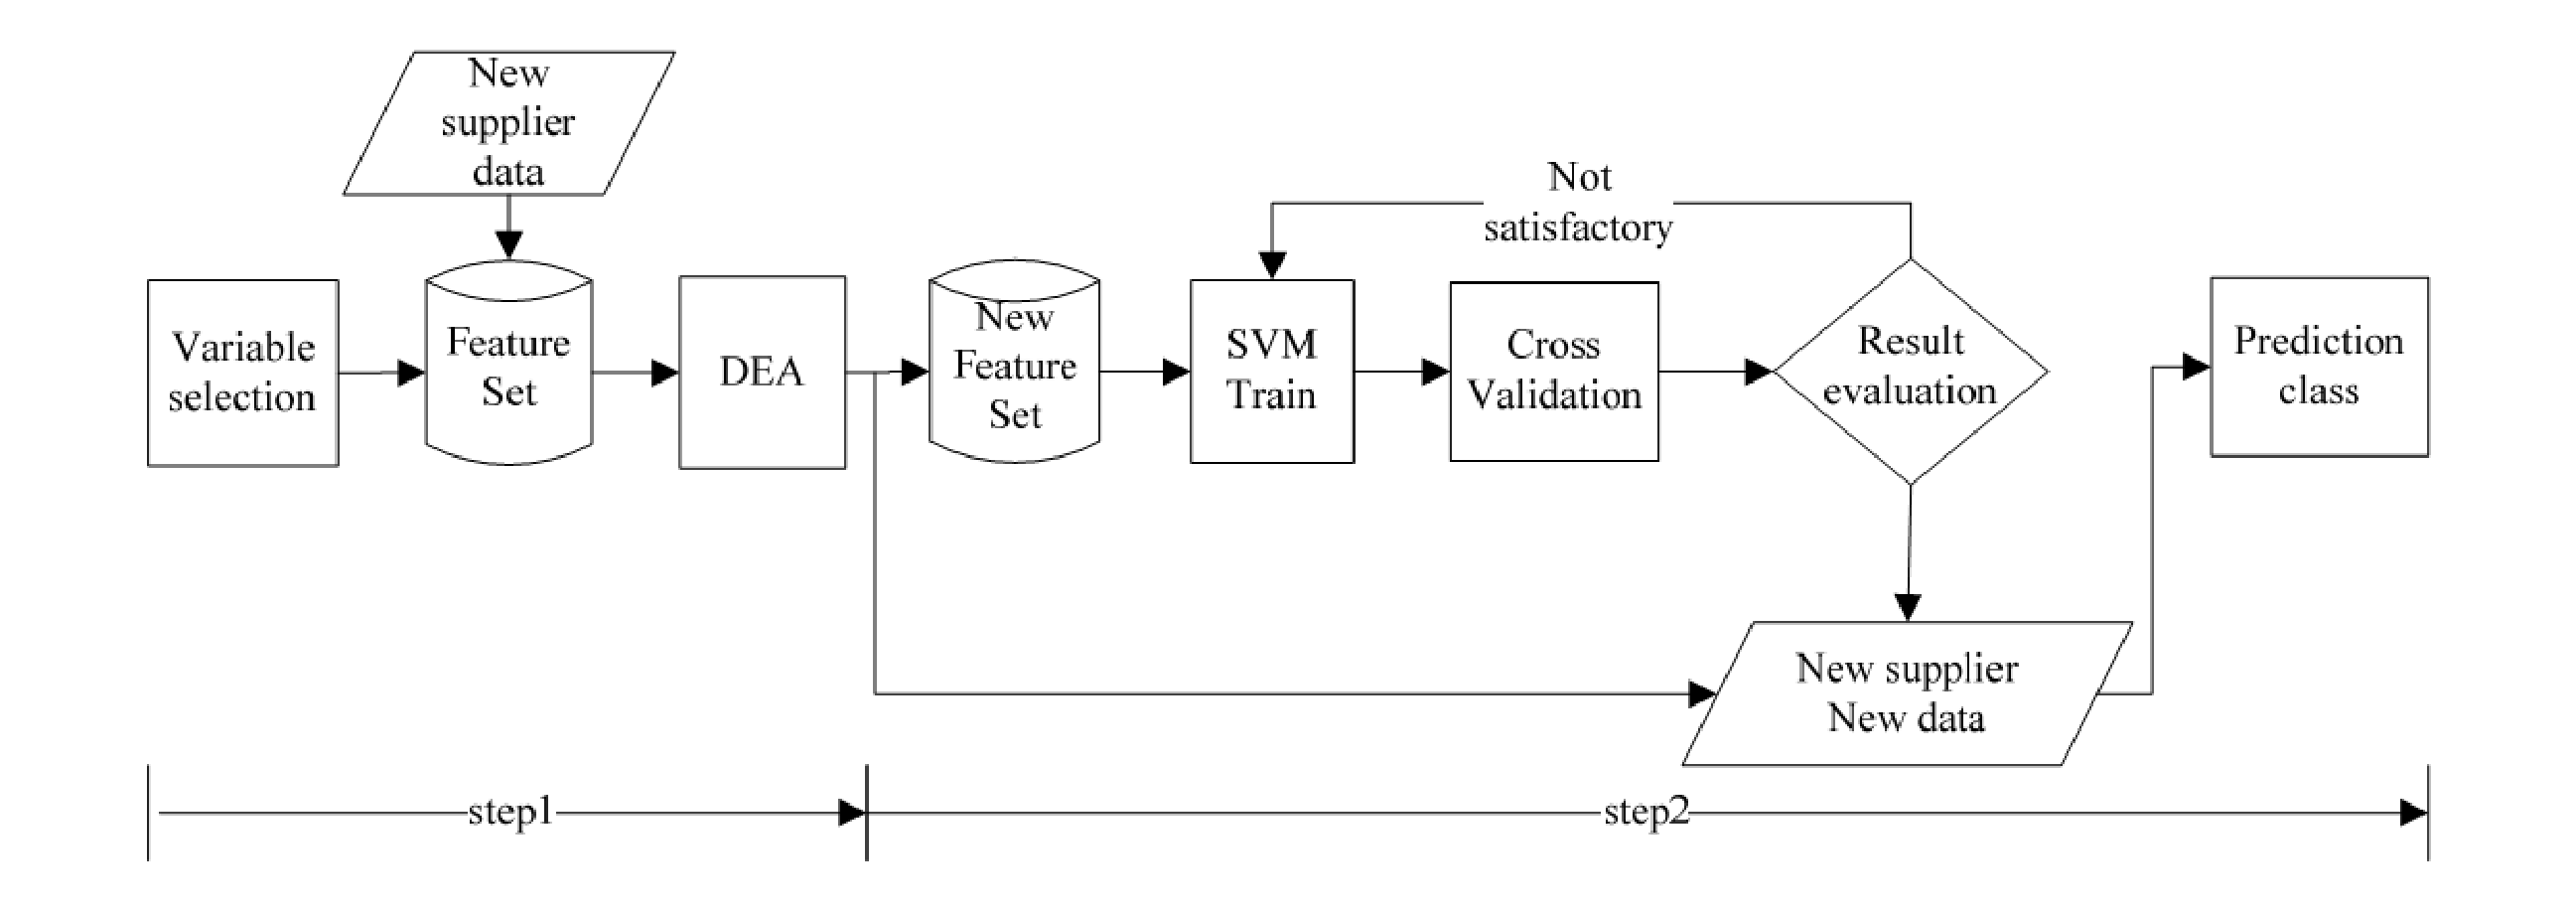
\includegraphics[width=0.85\textwidth,height=4cm]{figures/deasvm.eps}
  \caption{DEA-SVM混合模型}\label{fig:deasvm}
\end{figure}

DEA模型天生就是一个分类器,无需建立输入输出之间显性的函数关系,就可以将决策单元划分为两组:相对有效的决策单元(相对效率值等于1)、相对无效的决策单元(相对效率值小于1)。研究人员已经开始研究数据包络分析模型自然分类的能力,融合机器学习中经典的分类方法,如支持向量机(SVM),构建集成形式的分类器\cite{rezaie2013integrated,jiang2013supplier}。无论是直接利用相对效率值实现自动标记\cite{rezaie2013integrated},还是将相对效率值作为新的独立特征引入数据集\cite{jiang2013supplier},都取得良好的表现。

由传统DEA方法产生的生产前沿面实际上可以看做一个分段生产函数(Piecewise Production Function),Po等人\cite{po2009cluster}根据据此对决策单元做聚类分析。

通常,关联规则的兴趣度可以使用支持度和置信度两个指标度量。然而,在实际生活中,能够反映兴趣度的因素可能有多个,使得关联规则评价变成多属性决策问题。于是,Chen\cite{chen2007ranking}、Toloo等人\cite{toloo2009discover}使用DEA方法解决关联规则挖掘问题。

\section{基于数据包络分析的排名模型}
对于前沿面上相对有效的DMU,原始的DEA模型没有提供更多的信息区分它们,从而无法得到所有DMU 的完全排名(Full Ranking)结果。如果能够提升DEA的区分能力,则完全排名的问题就可以迎刃。在传统的DEA模型中,每个DMU都存在一个相对整个DMU集合,对于自身最佳的权值,由此确定了各个DMU相对于整个DMU集合的相对效率值。如果能够从整个DMU集合出发,寻找最佳的DMU作为参考,从而可以确定一个公共权值(Common Weight),作为衡量各个DMU“绝对效率”的标准,从而实现完全排名的目的。

关于公共权值和排名问题,目前已经有很多研究人员参与研究。1990年,Cook等人\cite{cook1990data}首次提出公共权值的概念。1991年,Roll等人
\cite{roll1991controlling}首次使用公共权值评价高速路养护单位。Cook和Kress\cite{cook1990data,cook1991multiple}通过缩小权值上下界的差距,利用有界DEA的公共权值给出主观有序偏好排名。Cook等人\cite{cook1992prioritization},Andersen和Petersen\cite{andersen1993procedure}分别发展了排列相对有效决策单元的过程。Ganley与Cubbin\cite{ganley1992public}通过最大化所有DMU的效率分值之和,确定一个公共权值用于对各个决策单元排名。Doyle 和Green \cite{doyle1994efficiency} 利用交叉效率矩阵发展了一种排名尺度方法(Rank Scale Method)。Sinuany–Stern等人\cite{sinuany1994academic}引入了包括两阶段线性判定分析(Two-stage Linear Discriminate Analysis)在内的多种分析方法对DMU集合进行排名。Cooper和Tone 通过计算基于松弛变量的相对效率值,使用其中相对无效的效率值尺度度量进行排名\cite{cooper1997measures}。Liu和Peng\cite{liu2008rankingdea}提出公共权值分析(Common Weights Analysis, CWA)的概念,利用公共权值集合,可以预计算相对有效的DMU的绝对效率分值,即构建一条隐含的绝对效率前沿面作为标准参照。

近年来,利用DEA方法对决策单元进行效率排序的方法层出不穷\cite{adler2002review,rita2011ranking},如交叉效率评价方法\cite{sexton1986data},超效率排名技术
\cite{andersen1993procedure},融合多目标决策(MCDM)的数据包络分析方法\cite{jahanshahloo2005note}等,得到长足的发展与广泛的应用。

\subsection{交叉评价方法}
在传统DEA模型,如CCR模型中,各DMU都选择对于自己最有利的权值,不同DMU拥有不同的最优权值,导致相互之间的效率失去可比性,传统DEA单纯依靠自评体系来评价决策单元有失公允。Sexton 等人\cite{sexton1986data}充分利用所有DMU的评价信息,通过建立交叉评估矩阵(Cross-Evaluation Matrix),利用平均交叉效率值,对DMU 进行优劣评价和排名。交叉效率评价方法希望利用互评体系来弥补自评体系的缺陷。

对于任意两个决策单元$\mathrm{DMU_i}$和$\mathrm{DMU_j}$,交叉效率评价方法执行以下几个步骤:
\begin{enumerate}[(1)]
  \item 计算各自的相对效率$h_i = h_{ii}$、$h_j = h_{jj}$。
  \item 计算交叉效率$h_{ij}$、$h_{ji}$,对于$h_{ji}$,可以通过下面条件DEA模型确定:
\begin{equation}\label{eq:ce1}
\begin{array}{ll}
  h_{ji} = & \max\limits_{\mu} \mu^T y_i\\
  \textit{s.t.} & h_{jj}\nu^Tx_j - \mu^Ty_j = 0 \\
   & \nu^Tx_i - \mu^Ty_i \ge 0 \\
   & \nu^Tx_i = 1 \\
   & \nu\ge 0
\end{array}
\end{equation}
由第一个约束条件可知,可行解源于决策单元$\mathrm{DMU_j}$的最优权值,反映决策单元$\mathrm{DMU_j}$对输入、输出指标的评价,而目标函数$\mu^T y_i$则反映了$\mathrm{DMU_j}$对$\mathrm{DMU_i}$的评价。$h_{ji}$的计算方法类似。
  \item 使用交叉效率构造交叉效率矩阵:
\begin{equation}
H=
\begin{bmatrix}
h_{11} & h_{12} & \cdots & h_{1n}\\
h_{21} & h_{22} & \cdots & h_{2n}\\
\vdots & \vdots & \ddots & \vdots\\
h_{n1} & h_{n2} & \cdots & h_{nn}\\
\end{bmatrix}
\end{equation}\label{eq:cem}
由此,可以获得决策单元$\mathrm{DMU_k}(k = 1,\ldots,n)$的平均效率\cite{doyle1994efficiency}:
\begin{equation}\label{eq:averageefficiency}
  \begin{array}{lll}
    \bar{h}_k  & = & \frac{1}{n}\sum\limits_{j=1}^nh_{kj} (Averaged~Appraisal~\textbf{of}~Peers)\\
    \bar{h}_k & = & \frac{1}{n}\sum\limits_{i=1}^n h_{ik} (Averaged~Appraisal~\textbf{by}~Peers)
  \end{array}
\end{equation}
由于平均效率是全部决策单元共同表决的结果,因此可作为各个决策单元排名的依据。
\end{enumerate}

交叉效率评价方法依然存在缺陷,如交叉效率值不唯一;平均交叉效率值和权重之间没有相应的联系,无法帮助决策者改进其效率;最终的平均交叉效率值并非帕累托最优或是可以进行帕累托改进,无法使所有的决策单元确信接受最终的评价结果。对于交叉效率评价方法的一些缺陷,陆续有研究人员提出改进。比如,Doyle 等人
\cite{doyle1994efficiency}使用全局优化技术,以确定出全局最优解,确保最优解是唯一的。

交叉效率评价方法的应用比较丰富,比如对夏季奥林匹克运动会参赛国家进行排名\cite{de2008cross,de2009ranking,wu2009achievement}。

\subsection{超效率排名模型}
利用传统DEA方法评估决策单元,通常存在多个相对有效的决策单元,无法直接利用相对效率值对相对有效的决策单元做进一步区分。为了弥补这一不足,Banker与Gifford\cite{banker1988relative}首次提出将有效决策单元从效率前沿面分离开来,在CCR模型的基础上构建超效率DEA模型,度量各决策单元的超效率分值。在Andersen 与Petersen\cite{andersen1993procedure}的努力下,得到进一步完善。超效率模型(Super Efficiency Model)的基本思想:将待评测决策单元的投入和产出使用其它所有单元的投入和产出的线性组合替代,而将被评测单元排除在参考集(Reference Set)之外来评估其效率。
\begin{equation}\label{eq:superefficiency}
  \begin{array}{lllll}
    \max & \mu^T y_k & & \min & \theta\\
    \textit{s.t.} & \nu^T x_i - \mu^T y_i \ge 0 & & \textit{s.t.} & \sum\limits_{i=1}^n \lambda_i x_i \le \theta x_k\\
    & \nu^T x_k = 1 & & & \sum\limits_{i=1}^n \lambda_i y_i \ge y_k\\
    & \nu \ge 0,\mu \ge 0 & & & \lambda_i \ge 0\\
    & i = 1,\ldots, n , i \ne k &&& i = 1,\ldots, n, i \ne k
  \end{array}
\end{equation}
对于无效决策单元,超效率模型估计的结果与CCR模型结果一致;对于CCR模型下有效的决策单元,在超效率模型下效率值$\theta$一般都是大于1。超效率DEA模型的经济含义是:一个有效决策单元可以将其投入按比例增加而效率值保持不变,投入增加的最大比例就是其超效率值$\theta - 1$。

超效率模型存在一个不足:使用传统CCR模型确定的相对有效的决策单元,在超效率模型中可能无可行解。对此,Lovell与Rouse\cite{lovell2003equivalent}提出一个新的超效率模型解决这一问题,确保所有决策单元都有可行解。

\subsection{公共权值向量集}
传统的DEA方法允许每个决策单元选择最有利于自身的指标权值向量,作为评价其生产效率的基准,由此确立的各个决策单元的相对效率缺乏可比性,无法作为决策单元排名的依据。为了对所有的决策单元采用统一的标准进行评估,研究人员便提出公共权值向量集(Common Set of Weights)的概念。公共权值向量集解自多目标规划,是生产可能集(Production Possibility Set, PPS)
\footnote{PPS将决策单元分成两组:处于PPS内的是无效率的决策单元,位于PPS前沿面上的是有效的决策单元。}
支持超平面(Supporting Hyperplane)的法向量(Normal Vector)。 使用公共权值向量集对决策单元进行排名是一个重要的方法,对决策单元进行排名需要首先定义一个度量决策单元与超平面距离的范数\cite{cook1990dea,roll1991controlling,cook2007within,liu2008ranking,payan2011modified}。

\cite{li2000ranking}利用决策单元集合构造输入最小输出最大的虚拟决策单元,根据CCR模型确定虚拟决策单元的最大效率,从而解得其最优权值作为公共权值,据此可以评估各个决策单元的相对效率,并进行效率排名。

\subsection{DR/DEA方法}
根据DEA模型计算的相对效率可以将决策单元分成两个类簇:相对有效的($\mathcal{P}$)与相对无效的($\mathcal{N}$),Sinuany-Stern和Friedman\cite{sinuany1998dea}根据两个类簇定义了一个比率分值
\begin{equation}\label{eq:dr}
  T_i = \frac{\mu^T y_i}{\nu^T x_i}, i = 1,\ldots, n
\end{equation}
并基于“最大化类簇间比率分值差异,最小化类簇内比率分值差异”的原则,寻找最佳公共权值向量,作为分离两个类簇决策单元的分类函数。对于类簇$\mathcal P$ 与$\mathcal N$,各自的平均比率分值定义为:
\begin{equation}
  \begin{array}{lll}
    \bar{T}_\mathcal{P} & = & \frac{1}{n_1} \sum\limits_{i\in \mathcal{P}} T_i \\
    \bar{T}_\mathcal{N} & = & \frac{1}{n_2} \sum\limits_{i\in \mathcal{N}} T_i
  \end{array}
\end{equation}
其中,$n_1,n_2$分别表示类簇$\mathcal{P},\mathcal{N}$的大小。由此可以确定所有决策单元平均比率分值:
\[
 \bar{T} = \frac{n_1\bar{T}_\mathcal{P} + n_2\bar{T}_\mathcal{N}}{n}
\]

选择最佳公共权值向量转化为如下最优化问题:
\begin{equation}
  \max_{\mu,\nu} \lambda = \frac{SS_B(T)}{SS_W(T)}
\end{equation}
其中,$SS_B(T),SS_W(T)$表示类簇间(内)比率分值差异,定义为:
\begin{equation}
  \begin{array}{lll}
    SS_B(T) & = & n_1(\bar{T}_\mathcal{P} - \bar{T})^2 + n_2(\bar{T}_\mathcal{N} - \bar{T})^2 = \frac{n_1n_2}{n_1+n_2}(\bar{T}_\mathcal{P} - \bar{T}_\mathcal{N})^2\\
    SS_W(T) & = & \sum\limits_{i\in \mathcal{P}} (T_i - \bar{T}_\mathcal{P})^2 + \sum\limits_{i\in \mathcal{N}} (T_i - \bar{T}_\mathcal{N})^2
  \end{array}
\end{equation}

DR/DEA属于非线性优化问题,\cite{sinuany1998dea}使用的共轭梯度算法(Conjugate Gradient Algorithm)优化模型,但无法保证能够找到全局最优解。

利用最优公共权值,可以实现对所有决策单元进行完全排序,并保证相对有效的决策单元排列在无效决策单元之前。

\subsection{基于切比雪夫距离的排名方法}
Tavares与Antunes\cite{tavares2001atchebycheff}提出一种类似于加法模型的效率评价方法,唯一的区别就是最小化被评价单元与有效前沿面的$L_{\infty}$范数距离(也称切比雪夫距离,或棋盘距离):
\begin{equation}\label{eq:chebycheffmodel}
  \begin{array}{ll}
    \min & \|(x_k, y_k) - (\sum\limits_{i=1}^n \lambda_i x_i,\sum\limits_{i=1}^n \lambda_i y_i)\|_{\infty}\\
    \textit{s.t.} & x_k \ge \sum\limits_{i=1}^n \lambda_i x_i \\
    & y_k \le \sum\limits_{i=1}^n \lambda_i y_i\\
    & \sum\limits_{i=1}^n \lambda_i = 1\\
    & \lambda_i \ge 0, i =1,\ldots, n
  \end{array}
\end{equation}
可以证明,模型\eqref{eq:chebycheffmodel}等价于下面的线性模型\cite{rezai2012ranking}:
\begin{equation}\label{eq:chebycheffmodel-eqv}
  \begin{array}{ll}
    \max & u_k\\
    \textit{s.t.} & x_k \ge \sum\limits_{i=1}^n \lambda_i x_i + u_k \\
    & y_k \le \sum\limits_{i=1}^n \lambda_i y_i - u_k\\
    & \sum\limits_{i=1}^n \lambda_i = 1\\
    & \lambda_i \ge 0, i =1,\ldots, n
  \end{array}
\end{equation}
其中,$u_k\in [0,\infty)$表示效率值,当且仅当$u_k =0$时,决策单元$\mathrm{DMU_k}$是有效的,或者取$\theta_k = 1/(1+u_k)$,当$\theta_k = 1$时,决策单元有效。

\cite{rezai2012ranking}将待评测的决策单元从生产可能集中剔除,使用下面的模型计算其效率值:
\begin{equation}
  \begin{array}{ll}
    \min & \|(x_k,y_k) - (\sum\limits_{i=1, i \ne k}^n \lambda_i x_i,\sum\limits_{i=1, i \ne k}^n \lambda_i y_i)\|_{\infty} \\
    \textit{s.t.} & x_k \le \sum\limits_{i=1, i \ne k}^n \lambda_i x_i \\
    & y_k \ge \sum\limits_{i=1, i \ne k}^n \lambda_i y_i\\
    & \lambda_i \ge 0, i =1,\ldots, n
  \end{array}
\end{equation}

根据$L_{\infty}$的定义可知:
\begin{equation}\label{eq:infinitynorm}
  \begin{array}{ll}
     & \|(x_k,y_k) - (\sum\limits_{i=1, i \ne k}^n \lambda_i x_i,\sum\limits_{i=1, i \ne k}^n \lambda_i y_i)\|_{\infty} \\
     = & \max\bigg\{\big\{|x_{kl} - \sum\limits_{i = 1, i\ne k}^n \lambda_i x_{il}|\big\}_{l=1}^m,\big\{|y_{kr} - \sum\limits_{i = 1, i\ne k}^n \lambda_i y_{ir}|\big\}_{r=1}^s\bigg\} \\
     = & \max\bigg\{\big\{\sum\limits_{i = 1, i\ne k}^n \lambda_i x_{il} - x_{kl}\big\}_{l=1}^m,\big\{y_{kr} - \sum\limits_{i = 1, i\ne k}^n \lambda_i y_{ir}\big\}_{r=1}^s\bigg\}\\
     \triangleq & v_k
  \end{array}
\end{equation}
则有下面模型:
\begin{equation}
  \begin{array}{ll}
    \min & v_k \\
    \textit{s.t.} & v_k \ge \sum\limits_{i=1, i \ne k}^n \lambda_i x_i - x_k\\
    & v_k \ge y_k - \sum\limits_{i=1, i \ne k}^n \lambda_i y_i\\
    & \lambda_i \ge 0, i =1,\ldots, n
  \end{array}
\end{equation}
根据对偶理论,可得其对偶模型:
\begin{equation}
  \begin{array}{ll}
    \max & \mu^T y_k - \nu^T x_k\\
    \textit{s.t.} & \mu^T y_i \le \nu^T x_i\\
    & 1^T \mu + 1^T \nu = 1\\
    &\mu \ge 0, \nu \ge 0\\
    & i = 1,\ldots, n, i \ne k
  \end{array}
\end{equation}

\subsection{PCA排名}
Joe Zhu\cite{zhu1998data}做过关于DEA与PCA两种方法的比较实验,发现二者对决策单元的排名具有一致性。后来,Premachandra\cite{premachandra2001note}对Zhu的方法做了进一步的改进。

\chapter{AHP}
20世纪中后期,美国运筹学家Saaty\cite{saaty1977scaling,saaty1980analytic}提出了层次分析法(Analytic Hierarchy Process,简称AHP)。它是一种定性与定量相结合的、系统的、层次化的,能够有效解决多准则多目标问题分析方法,主要用于解决复杂的决策、评价、分析和预测问题。AHP应用比较广泛,可解决人力资源管理\cite{saaty2007analytic}、医学诊断\cite{saaty1998diagnosis}、经济计划与管理、能源政策与分配、生产决策、交通运输、预测等问题
\cite{ercsan2012use} 等。

AHP将决策问题分解为子问题,建立一种层次化的结构,通过逐层分析,确定最佳的备选方案。从心理学的角度来看,AHP将决策问题理性地拆分,从不同层面理解决策者的意图,并运用各个层面之间的内在联系,寻找最能契合决策者目标的方案。一般地,AHP将决策问题分为三个层次:目标层(Goal)、准则层(Criteria)和方案层(Alternatives)。

\begin{example}
决策者需要从桂林、黄山、北戴河三个目的地选择一个作为度假旅游的去处,那么按照正常的思路,她(他)会根据景色、餐饮、居住、行程等多个因素综合分析,并确定最终的方案。这个决策问题的目标即确定一个旅游目的地,而方案就三个:桂林、黄山与北戴河,而准则就是决策者选择方案所考虑的因素,包括景色、餐饮、居住、行程等。据此,AHP建立如图~\ref{fig:ahp}所示形式的层次关系图
\footnote{\href{http://www.math.zju.edu.cn/ligangliu/Courses/MathematicalModeling\_2005-2006/Syllabus/chapter\_12.pdf}{浙江大学数学建模课程}}。
\begin{figure}[htbp]
\centering
\fbox{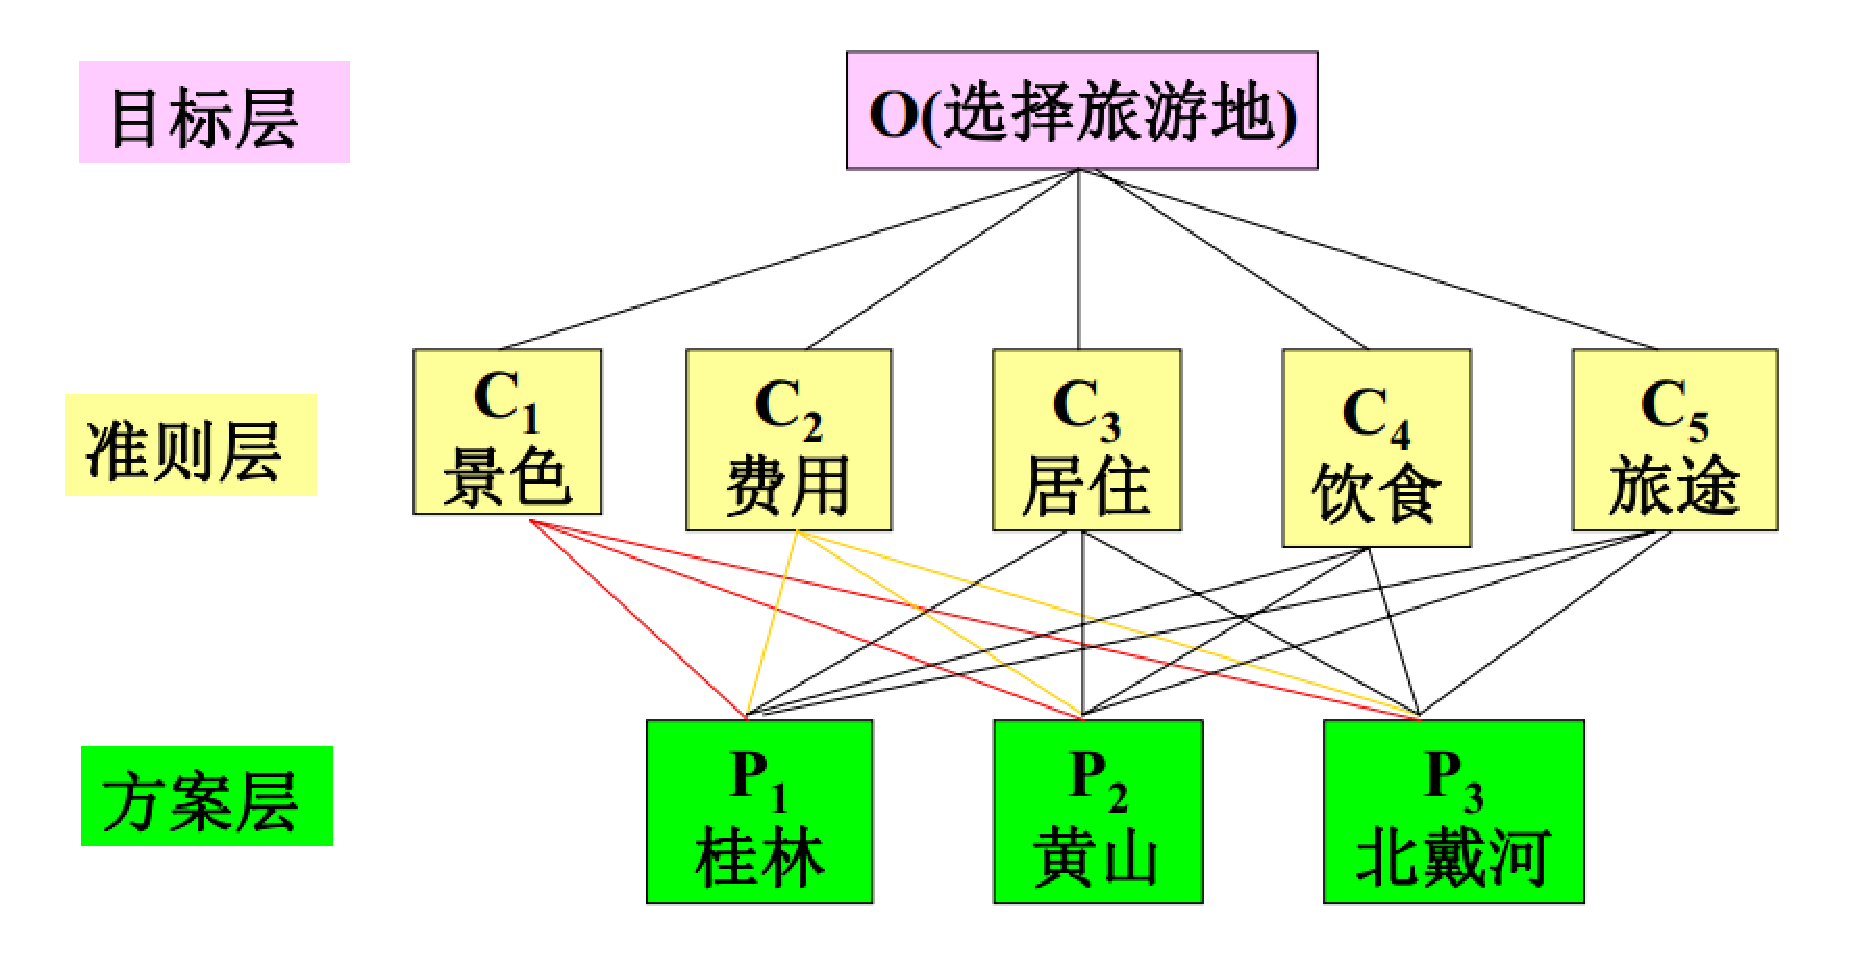
\includegraphics[width=0.8\textwidth, height=6cm]{figures/AHP.eps}}
\caption{Analytic Hierarchy Process: Decision on a Vacation Spot}
\label{fig:ahp}
\end{figure}
\end{example}

\section{基本步骤}
AHP确立层次结构以后,会根据各个准则相对于目标的重要程度做两两比较,然后根据各个方案对于各项准则的权重量化准则和方案层。尔后,根据两组权重综合确定各方案对目标的权重。具体包含以下几个步骤:
\begin{enumerate}[(1)]
\item 建立层次分析结构模型,如图\ref{fig:ahp}所示。
\item 构造判断矩阵。使用序对比较法和$1\sim 9$尺度,构造每层相对上一层各个因素的判断矩阵。
\item 计算权向量并作一致性检验。对每个判断矩阵计算最大特征值和特征向量,作一致性检验,若通过,则特征向量即权重向量,否则重新构造判断矩阵。
\item 计算组合权重向量。如果组合权向量通过一致性检验,则可以作为决策的依据,否则重新构造一致性较弱的判断矩阵。
\end{enumerate}
根据基本步骤,我们在下文尝试着解决前述旅游景点选择问题。

\subsection{构造判断矩阵}
根据各个准则$c_1,\ldots,c_n$相对目标$O$的重要程度,决策者对准则层两两比较,任选准则$c_i$和$c_j$,确定相对权值$a_{ij}$。为了方便从定性到定量的转化,Saaty提出使用$1\sim 9$尺度,即$1\le a_{ij} \le 9$,或者尺度$1\sim 9$的倒数。相对权值构成判断矩阵$A=(a_{ij})_{n \times n}$,且满足$a_{ij}=1/a_{ji},a_{ii} = 1,i,j=1,\ldots,n$,因此$A>0$ 是正互反矩阵(Positive Reciprocal Matrix)。
\begin{equation}
A=
\begin{bmatrix}
    1 & 1/2 & 4 & 3 & 3\\
    2 & 1 & 7 & 5 & 5\\
    1/4 & 1/7 & 1 & 1/2 & 1/3\\
    1/3 & 1/5 & 2 & 1 & 1\\
    1/3 & 1/5 & 3 & 1 & 1
\end{bmatrix}
\end{equation}

对于任意三个准则$c_i$、$c_j$和$c_k$,$i,j,k = 1,2,\ldots,n$,两两比较得到相对权值$a_{ij},a_{ik},a_{jk}$,如果满足$a_{ik}=a_{ij}a_{jk}$,则称判断矩阵$A$ 是一致矩阵。此时,可以认为决策者的判断行为是可信的、严格一致的\cite{saaty2003decision}。如果判断矩阵是一致矩阵,可以认为决策者严格根据自身对于各个元素相对上一层的相对权值进行判断。这种关系可以从数学上予以证明。

假如决策者认为准则$c_1,\ldots,c_n$相对目标$O$的重要程度分别为$w_1,\ldots,w_n$,据此对元素两两比较,得到相对权值$a_{ij}=w_i/w_j$,由此构造的判断矩阵
\begin{equation}
A=
\begin{bmatrix}
    w_1/w_1 & w_1/w_2 & \cdots & w_1/w_n\\
    w_2/w_1 & w_2/w_2 & \cdots & w_2/w_n\\
    \vdots & \vdots & \ddots & \vdots\\
    w_n/w_1 & w_n/w_2 & \cdots & w_n/w_n
\end{bmatrix}
\end{equation}\label{eq:prm}
是一致矩阵。

由于$A=\alpha\beta^T$,其中
\[\alpha = (w_1,w_2,\ldots,w_n)^T,~~~\beta = (\frac{1}{w_1},\frac{1}{w_2},\ldots,\frac{1}{w_n})^T\]

因此,矩阵$A$的秩为1,并且由于$A\alpha=\alpha\beta^T\alpha=n\alpha$,表明矩阵$A$存在唯一的非负特征值$n$,对应的特征向量$\alpha$,正是准则层相对目标层的相对权值。

\subsection{一致性检验}
一致性的判断终究只是一个理想的假设,实际上,决策者在决策时,比较合理也是可行的一种方式是两两比较,而直接对准则层构造一个权值列表是困难的。对于一个包含了$n$个元素的准则层,只需做$\binom{n}{2}$次序对比较,即可构造出决策者的判断矩阵。

在构造判断矩阵时,AHP允许一定程度的不一致性,但不一致性不能偏离过大以致判断行为不可信。为了衡量判断矩阵的一致性,Alexander和Saaty提出一致性检验的基本步骤\cite{alexander1977forward}:
\begin{enumerate}[(I)]
\item 计算一致性指标CI:
\[
    \textrm{CI} = \frac{\lambda_{\max}-n}{n-1}
\]
CI越大表明判断矩阵不一致性越严重,$\lambda_{\max}$是判断矩阵主特征值,可以证明$\lambda_{\max}\ge n$,且当$\lambda_{\max}=n$,从而CI=0,判断矩阵是一致性矩阵。

\item 计算平均随机一致性指标RI:
\begin{table}[ht]
\caption{Saaty's RI}\label{tbl:ri}
\centering
\begin{tabular}{r|ccccccccccc}
\hline
$n$ & 1 & 2 & 3 & 4 & 5 & 6 & 7 & 8 & 9 & 10 & 11\\
\hline
$RI$ & 0 & 0 & 0.58 & 0.90 & 1.12 & 1.24 & 1.32 & 1.41 & 1.45 & 1.49 & 1.51\\
\hline
\end{tabular}
\end{table}
表\ref{tbl:ri}是Alexander和Saaty的模拟结果,通过多次模拟生成判断矩阵,计算一致性指标CI,将多次模拟结果取平均。

\item 计算一致性比率CR:
\[
    \text{CR} = \frac{\text{CI}}{\text{RI}}
\]
根据Alexander和Saaty的模拟结果,认为当$\text{CR}<0.1$,则通过一致性检验。实际上这个阈值从理论上很难给出严格的证明,只是一种粗糙的估计,并引发了诸多争议。
\end{enumerate}

针对上例,通过计算可知$\lambda_{\max}=5.073$,对应特征向量为
\[
\omega^{(2)}=(0.263,0.475,0.055,0.090,0.110)^T.
\]
矩阵的一致性指标$\text{CI}=(5.073-5)/4=0.018$,查表\ref{tbl:ri}可知$\text{RI}=1.12$,一致性比率$\text{CR}=0.016<0.1$,表明矩阵$A$通过一致性检验。由此确定准则层相对目标层的权值向量$\omega^{(2)}\in \mathbb R^n$。

同理,可以确定相对某个准则,方案层的相对权值向量列表如下:
\[
    (0.595,0.277,0.129)^T,(0.082,0.236,0.682)^T,(0.429,0.429,0.142)^T,
\]
\[
    (0.633,0.193,0.175)^T,(0.166,0.166,0.668)^T,
\]
并且都通过了一致性检验。

\subsection{组合权重和组合一致性检验}
组合权重是指根据各准则相对目标的权重向量和各方案相对每一准则的权重向量计算的各个方案相对目标的权重向量。

根据确定的相对某个准则,方案层的相对权值向量,可以确定各个方案$a_1,\ldots,a_m$相对准则层的权值向量
$\omega_1^{(3)},\ldots,\omega_m^{(3)}\in \mathbb{R}^n$。根据上例确定的三个方案相对准则层(5个准则)的相对权值分别为:
\[\omega_1^{(3)}=(0.595,0.082,0.429,0.633,0.166)^T\]
\[\omega_2^{(3)}=(0.277,0.236,0.429,0.193,0.166)^T\]
\[\omega_3^{(3)}=(0.129,0.682,0.142,0.175,0.668)^T\]
根据准则层相对目标层的权值$\omega^{(2)}$,以及方案层相对准则层的相对权值$\omega_1^{(3)},\omega_2^{(3)},\omega_3^{(3)}$可以确定各个方案相对目标的最终权值。
\begin{itemize}
\item 桂林相对目标的权值为
\[\omega_1 = (0.595,0.082,0.429,0.633,0.166)(0.263,0.475,0.055,0.090,0.110)^T=0.3\]
\item 黄山相对目标的权值为
\[\omega_2 = (0.277,0.236,0.429,0.193,0.166)(0.263,0.475,0.055,0.090,0.110)^T=0.246\]
\item 北戴河相对目标的权值为
\[\omega_3 = (0.129,0.682,0.142,0.175,0.668)(0.263,0.475,0.055,0.090,0.110)^T=0.456\]
\end{itemize}
如果通过组合一致性检验,根据计算可知,决策者最终会选择北戴河作为旅游目的地。

下文主要介绍如何做组合一致性检验。组合一致性检验需要逐层进行,假设第1层只有一个元素,即单目标情形,第$k$层对第$k-1$层的一致性指标为$\mathrm{CI}_1^{(k)},\mathrm{CI}_2^{(k)},\ldots,\mathrm{CI}_{n_{k-1}}^{(k)}$,随机一致性指标为$\mathrm{RI}_1^{(k)},\mathrm{RI}_2^{(k)},\ldots,\mathrm{RI}_{n_{k-1}}^{(k)}$,其中$n_{k-1}$是第$k-1$ 层元素的个数,则第$k$层对第$1$层的组合一致性指标定义为:
\[\mathrm{CI}^{(k)} = (\mathrm{CI}_1^{(k)},\mathrm{CI}_2^{(k)},\ldots,\mathrm{CI}_{n_{k-1}}^{(k)})\omega_{k-1}\]
组合随机一致性指标定义为:
\[\mathrm{RI}^{(k)} = (\mathrm{RI}_1^{(k)},\mathrm{RI}_2^{(k)},\ldots,\mathrm{RI}_{n_{k-1}}^{(k)})\omega_{k-1}\]
组合一致性比率定义为:
\[\mathrm{CR}^{(k)} = \mathrm{CR}^{(k-1)} + \frac{\mathrm{CI}^{(k)}}{\mathrm{RI}^{(k)}}\]
其中,$k=3,4,\ldots$

\subsection{判断矩阵主特征值}
由于判断矩阵是正互反矩阵,则其主特征值$\lambda_{\max}\ge n$,我们现在给出证明\cite{xu1988ahp}。

\begin{proof}
假设判断矩阵$A$主特征值是$\lambda_{\max}$,对应特征向量是$\omega = (\omega_1,\ldots,\omega_n)^T$,根据$A\omega = \lambda_{\max}\omega$,则对任意的
$i=1,2,\ldots,n$,都有
\[\lambda_{\max}\omega_i = \sum_{j=1}^n{a_{ij}\omega_j},\]
那么
\[\lambda_{\max}=\sum_{j=1}^n{a_{ij}\frac{\omega_j}{\omega_i}},\]
于是
\[\lambda_{\max}-1=\sum_{j=1}^n{a_{ij}\frac{\omega_j}{\omega_i}}-1=\sum_{j\neq i}{a_{ij}\frac{\omega_j}{\omega_i}},\]
由于
\[\sum_{j\neq i}{a_{ij}\frac{\omega_j}{\omega_i}}=S_1 + S_2,\]
其中,
\[
    S_1 = \sum_{1\le j< i}{a_{ij}\frac{\omega_j}{\omega_i}},~~S_2 = \sum_{i< j\le n}{a_{ij}\frac{\omega_j}{\omega_i}} = \sum_{j< i\le n}{a_{ji}\frac{\omega_i}{\omega_j}}
\]
所以有等式
\[n\lambda_{\max}-n=\sum_{i=1}^n{\sum_{j\neq i}{a_{ij}\frac{\omega_j}{\omega_i}}}=\sum_{1\le j<i\le n}({a_{ij}\frac{\omega_j}{\omega_i} + a_{ji}\frac{\omega_i}{\omega_j}})\]
由此可得
\[\lambda_{\max} = \frac{1}{n}\sum_{1\le j<i\le n}({a_{ij}\frac{\omega_j}{\omega_i} + a_{ji}\frac{\omega_i}{\omega_j}}) + 1\]
那么一致性指标$\mathrm{CI}$有:
\[
    \mathrm{CI} = \frac{1}{n(n-1)}\sum_{1\le j<i\le n}({a_{ij}\frac{\omega_j}{\omega_i} + a_{ji}\frac{\omega_i}{\omega_j}}) - 1
\]
要证$\lambda_{\max}>n$,只要证明$\mathrm{CI}>0$即可。

假设判断矩阵是一致性矩阵$\bar A=(\dfrac{\omega_i}{\omega_j})$扰动的结果,而且
\[
    a_{ij} = \frac{\omega_i}{\omega_j}\epsilon_{ij},\epsilon_{ij}>0,\forall i,j=1,2,\ldots,n
\]
则据此可得
\[
    \mathrm{CI} = \frac{1}{n(n-1)}\sum_{1\le j<i\le n}(\epsilon_{ij} + \frac{1}{\epsilon_{ij}}) - 1
\]
若令$\delta_{ij}=\epsilon_{ij}-1>-1,\forall i,j=1,2,\ldots,n$,则
\[
    a_{ij} = \frac{\omega_i}{\omega_j} + \frac{\omega_i}{\omega_j}\delta_{ij}
\]
表明$\delta_{ij}$可视为扰动比例。

将$\epsilon_{ij}=\delta_{ij}+1$代入一致性指标,则有
\[
    \mathrm{CI} = \frac{1}{n(n-1)}\sum_{1\le j<i\le n}(\delta_{ij} + 1 + \frac{1}{\delta_{ij}+1}) - 1=\frac{1}{n(n-1)}\sum_{1\le j<i\le n}{\frac{(\delta_{ij}+1)^2+1}{\delta_{ij}+1}-2}
\]
即
\[
    \mathrm{CI} = \frac{1}{n(n-1)}\sum_{1\le j<i\le n}{\frac{\delta_{ij}^2}{\delta_{ij}+1}}>0
\]
由此,证得$\lambda_{\max}>n$。\qedhere
\end{proof}

计算判断矩阵的主特征值和特征向量的方法有多种,如幂法、和积法、方根法都可以非常高效地完成计算。

\subsection{方根法}

\begin{enumerate}[(1)]
\item 计算判断矩阵每一行元素的乘积:
\[m_i = \prod_j a_{ij},i=1,2,\ldots,n\]

\item 计算$m_i$的$n$次方根:
\[\bar{w_i} = \sqrt[n]{m_i},i=1,2,\ldots,n\]

\item 对向量$\bar{w} = (\bar{w}_1,\bar{w}_2,\ldots,\bar{w}_n)^T$归一化处理:
\[w_i = \frac{\bar{w}_i}{\sum \limits_i \bar{w}_i}\]
则$w=(w_1,w_2,\ldots,w_n)^T$即为主特征向量。

\item 计算主特征值$\lambda_{max}$:
\[\lambda_{\max} = \sum_i \frac{(Aw)_i}{nw_i}\]
式中,$(Aw)_i$表示$Aw$的第$i$个元素。

\end{enumerate}

\subsection{和积法}
\begin{enumerate}[(1)]
\item 将判断矩阵每一列归一化:
\[\bar{a}_{ij} = \frac{a_{ij}}{\sum \limits_i a_{ij}},~~i,j = 1,2,\ldots,n\]

\item 将按列归一化后的判断矩阵按行相加:
\[\bar{w}_i = \sum_j \bar{a}_{ij},~~i=1,2,\ldots,n\]

\item 对向量$\bar{w} = (\bar{w}_1,\bar{w}_2,\ldots,\bar{w}_n)^T$归一化处理:
\[w_i = \frac{\bar{w}_i}{\sum \limits_{i=1}^n{\bar{w}_i}}\]
则$w=(w_1,w_2,\ldots,w_n)^T$即为主特征向量。

\item 计算主特征值$\lambda_{\max}$:
\[\lambda_{\max} = \sum_i {\frac{(Aw)_i}{nw_i}}\]
式中,$(Aw)_i$表示$Aw$的第$i$个元素。
\end{enumerate}

\section{AHP与排名}
\subsection{排名聚合}
\cite{de2010search}将AHP应用到搜索引擎排名聚合:(1)根据各个独立搜索引擎历史表现两两比较,构造搜索引擎的判断矩阵,根据AHP特征向量法确定各个搜索引擎的权值;(2)对于每个搜索引擎返回的搜索结果列表,对列表中的所有文档对,根据它们在列表中的排名或者分值构造文档判断矩阵,从而确定各自在列表中的权值;(3)对于每篇文档,根据其文档权值与搜索引擎自身的权重,确定其综合相关分值。

假设使用的独立搜索引擎是$\mathrm{SE_1},\ldots, \mathrm{SE_m}$,决策者根据它们的历史表现构造出判断矩阵$A_{\mathrm{SE}}$,计算其主最大特征向量$\alpha = (\alpha_1,\ldots, \alpha_m)$ 作为各个搜索引擎自身的权重;对于搜索引擎$\mathrm{SE_i}, i=1,\ldots, m$,假设其返回的搜索结果列表是$D_i = (d_{i1},\ldots, d_{in_i})$,对所有$n_i$个文档在列表中的排名或者分值建立文档判断矩阵$A$,利用相似的方法可以确定其各自在列表中的权值$\beta_i = (\beta_{i1},\ldots,\beta_{in_i})$。 对于任意的文档$d$,可能同时出现在多个搜索引擎的搜索结果列表中,则其最终相关性分值:
\begin{equation}
  s = \sum\limits_{i=1}^m I(d\in D_i) \alpha_i * \beta_d^i
\end{equation}
其中,$I(d\in D_i)$是判别函数,如果文档$d$出现在$D_i$中,则$I(d\in D_i) = 1$,否则$I(d\in D_i) = 0$。$\beta_d^i$表示文档在列表$D_i$中的权重。

LETOR2.0上的实验结果表明,基于AHP的排名聚合方法(AHP-Rank,AHP-Score)性能要优于Borda Fuse和Weighted Borda Fuse两种方法。

\subsection{因子排名}
Guo等人\cite{guo2012personalized}认为影响推文(Tweet)排名的因子主要有七种:评论次数、转发次数、发布时间、博主的粉丝数目、匹配的标签、是否进入热点榜单、博主是否经过实名认证,并提出一种基于AHP的推文排名方法(TweetRank)。TweetRank根据用户的偏好,对所有影响因子两两比较形成影响因子比较矩阵,使用比较矩阵的主特征向量作为各个影响因子的权值,实现个性化推文排名的目的。实验表明,相比单纯使用时间因素对博文排名,TweetRank与用户的个性化偏好更为吻合。

在排序学习问题中,每个文档特征都可以作为一个独立的排名函数,对文档进行排名。基于AHP,可以根据特征在训练集中各个检索词下的排名精度(性能),两两比较构造比较矩阵,根据AHP理论确定各个特征的权重,由此构建出简单的线性排名函数,简称\textbf{AHPRank}。

假设检索词集合是$Q = \{q_j\}_{j=1}^n$,对于检索词$q_j\in Q$,记特征$i$在检索词$q_j$上的排名精度是$e_{ij}$,那么全部特征在训练数据集检索词集合上的排名精度矩阵$E = (e_{ij})_{mn}$,其中$m$是文档特征维数。

对于任意两个特征$i_1,i_2$,它们各自在训练数据集上的排名精度是$E_{i_1} = (e_{i_1,1},\ldots, e_{i_1,n}), E_{i_2} = (e_{i_2,1},\ldots, e_{i_2,n})$,比较二者在所有检索词上的排名精度,使用下面的规则进行积分($j = 1,2,\ldots, n$):
\begin{equation}\label{eq:rating}
  b_{i_1, j}^{(i_1,i_2)} =
  \left\{
    \begin{array}{ll}
      1, & e_{i_1,j} \ge e_{i_2,j}, \\
      0, & e_{i_1,j} < e_{i_2,j}.
    \end{array}
  \right.
\end{equation}

根据特征$i_1$与$i_2$的排名精度比较,得到其在不同检索词上的积分结果,统计加和得到总的积分:
\begin{equation}
  b_{i_1}^{(i_1,i_2)} = \sum\limits_{j=1}^n b_{i_1, j}^{(i_1,i_2)}
\end{equation}
同理,可以得到特征$i_2$的积分结果$b_{i_2}^{(i_1,i_2)}$。

令
\begin{equation}
  a_{i_1,i_2} = \frac{b_{i_1}^{(i_1,i_2)}}{b_{i_2}^{(i_1,i_2)}}
\end{equation}
则可以构造得到成对比较矩阵$A = (a_{ij})_{m\times m}$,其中
\begin{equation}
  a_{ij} = \frac{b_i^{(i,j)}}{b_j^{(i,j)}}
\end{equation}

利用方根法或者和积法可以迅速计算得到矩阵$A$的主特征向量$\omega = (\omega_1,\ldots, \omega_m)$,那么特征$i$的权值就是$\omega_i$,由此可以用作在测试集上的线性排名函数对文档进行排名。对于任意文档$d$,假设其特征向量为$x$,AHPRank的预测分值为:
\[
 s = \omega^T x
\]

\subsection{AHP与成对比较}
假设存在$n$个方案,通过投票表决各自获得票数是$m_1,\ldots, m_n$,那么对于任意两个方案$A_i, A_j$,利用得票差值可以构造判断矩阵$A=(a_{ij})$,其中
\[
    a_{ij} = e^{m_i - m_j}
\]
那么,判断矩阵显然是一个正互反矩阵,并且满足一致性:
\[
    a_{ij} a_{jk} = e^{m_i - m_j}  e^{m_j - m_k} = e^{m_i - m_k} = a_{ik}
\]

对于文档检索问题,文档特征集构成准则层,文档集构成方案层,对于某个检索词,我们可以尝试利用AHP方法,从文档数据集中筛选并排列出同检索词最相关的文档。

\subsection{排序逆转}
所谓排序逆转(Rank Reversal)是指决策方法对同一决策方案给出自相矛盾的评价,比如在成对比较时,可能会从不同的角度得出$A\succ B$,$B\succ C$,$C\succ A$ 的结论。排序逆转存在多种类型,有时选作评价决策方法优劣的标准。

\chapter{ELECTRE}
ELECTRE方法在\cite{benayoun1966manual}中首次提出,借助于超越关系(Outranking Relation)评估包含多个决策准则的决策方案。在第一个ELECTRE I\cite{roy1968classement}诞生以后,陆续扩展了多个版本:ELECTRE I, II, III, IV, TRI与TOPSIS\cite{hwang1981multiple},各个版本适用的范围、操作的方法是不同的,比如ELECTRE I\cite{roy1968classement}和ELECTRE IS主要用于选择问题(Selection Problem),ELECTRE TRI主要用作指派问题(Assignment Problem),或者应用到序分类(Ordinal Classification)问题。ELECTRE II, III, IV 主要用于排序问题(Ranking Problem),其中ELECTRE II\cite{roy1971methode,bertier1973methode}是老版本,ELECTRE III\cite{roy1978electre}考虑了准则间的相对重要程度,也是同IV 的差异之处。

ELECTRE III具有以下几个特征:
\begin{enumerate}[(1)]
  \item 引入无差异阈值(Indifference Threshold)和偏好阈值(Preference Threshold)的概念,将决策问题的模糊性(不精确和不确定性)考虑进来。
  \item 不同于其他多目标求解方法,它不允许补偿(non-compensatory)。也就是说,当一种准则分值过低,它不能通过其他高分值的准则获得补偿。
  \item 允许不可比(incomparability)的情况,即给定两个备选方案,无法给出明确的偏好。
\end{enumerate}

\section{偏好模型}
偏好模型是基于偏好关系(Preference Relation)建立的,传统模型定义偏好关系:
\begin{itemize}
  \item Preference:$a>b \Leftrightarrow g(a)>g(b)$
  \item Indifference:$a=b \Leftrightarrow g(a)=g(b)$
\end{itemize}
当备选方案a、b差别很小,从而无法抉择,这种偏好模型显然不能满意地解决该问题。

ELECTRE方法中定义了两个重要概念:Threshold和OutRanking,对于偏好模型,还引入无差异阈值(Indifference Threshold)$q$,并重新定义偏好关系:
\begin{itemize}
  \item Preference:$a>b \Leftrightarrow g(a)- g(b) > q$
  \item Indifference:$a=b \Leftrightarrow |g(a)-g(b)|\le q$
\end{itemize}

由于这个模型为严格偏好(Strict Preference)与无差异(Indifference)明确划定了一个界限,在实际问题中二者之间仍然存在着模糊性,因此有必要为二者设置一个缓冲带。为此,ELECTRE又引入了偏好阈值(Preference Threshold) $p$,并将偏好关系细化为两个二元关系:强偏好(Strong Preference)与弱偏好(Weak Preference),定义如下形式的偏好模型:
\begin{itemize}
  \item Strong Preference:$a>b \Leftrightarrow g(a)-g(b)>p$
  \item Weak Preference:$a\succ b \Leftrightarrow q<g(a)-g(b)\le p$
  \item Indifference:$a=b \Leftrightarrow |g(a)-g(b)|\le q$
\end{itemize}

根据偏好模型,ELECTRE确定了Outranking关系:
\begin{itemize}
  \item Outranking:$a\succeq b \Leftrightarrow (a>b)\bigcup(a\succ b)\bigcup(a=b)$
\end{itemize}
由此可知:$a=b$等价于$a\succeq b, b\succeq a$。

如果$\overline{a\succeq b}$,且$\overline{b\succeq a}$,则$a$和$b$是无法比较的(Incomparability)。

\begin{figure}[ht]
  \centering
  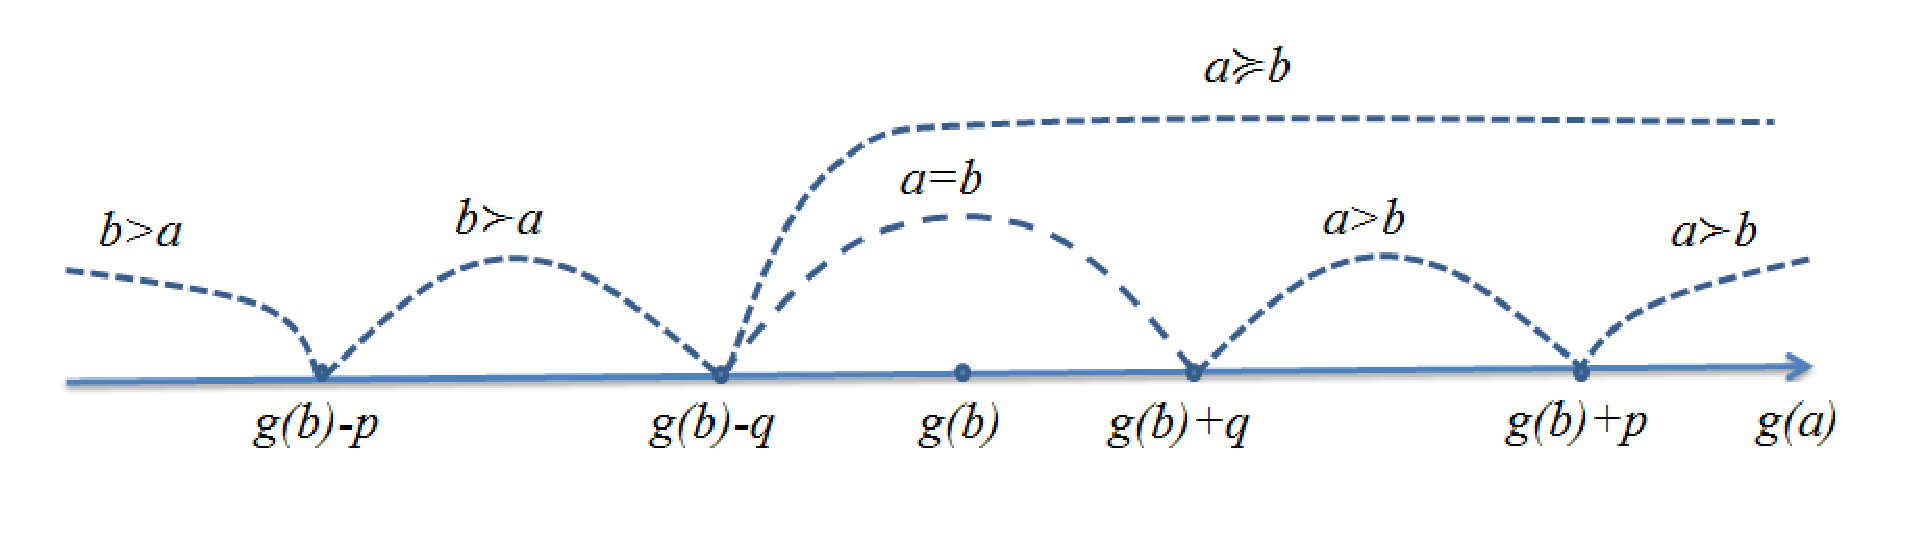
\includegraphics[width=0.8\textwidth]{figures/preferencerelation.eps}
  \caption{偏好关系}\label{fig:preferencerelation}
\end{figure}

\section{基本步骤}
假设某决策问题包含$m$个备选方案,方案集记为$A$;$n$个决策准则$g_j,j=1,2,\ldots,n$,准则集合记为$G$;每个决策准则对所有备选方案都能够做出评价,评价矩阵记为$X=(x_{ij})_{m\times n}$,$x_{ij}$表示决策准则$g_j$对备选方案$a_i$做出的评价,或者备选方案$a_i$在决策准则$g_j$上的得分。
从备选方案集$A$任选两个方案$(a_i,a_k)$,从准则集中任意一个准则$g_j$。

\subsection{确定阈值}
对准则$g_j$定义三种类型的阈值:无差异阈值$q_j$,偏好阈值$p_j$,否决阈值(Veto Threshold)$v_j$。一般而言,$0<q_j<p_j<v_j$,并根据给定条件判定方案$a_i$ 与$a_k$之间的关系:
\begin{enumerate}[(1)]
  \item 无差异:若$|x_{ij}-x_{kj} |\le q_j$,则认为在准则$g_j$下,方案$a_i$与$a_k$是无差异的
  \item 弱偏好:若$q_j<x_{ij}-x_{kj} \le p_j$,则认为在准则$g_j$下,方案$a_i$略优于$a_k$
  \item 强偏好:若$p_j<x_{ij}-x_{kj}$,则认为在准则$g_j$下,方案$a_i$优于$a_k$
  \item 否决:若$x_{ij}-x_{kj}\le -v_j$,则总体上,不再承认方案$a_i \succeq a_k$
\end{enumerate}

\subsection{计算一致优先度、非一致优先度}
一致优先度表示一个备选方案优于另一备选方案的程度。对于准则$g_j$,备选方案$a_i$优于方案$a_k$的一致优先度$c_j(i,k)$可以表示为下式:
\begin{equation}\label{eq:consistent}
  c_j(i,k)=\left\{
           \begin{array}{ll}
             0, & x_{ij}-x_{kj}\le -p_j, \\
             1, & x_{ij}-x_{kj}\ge -q_j, \\
             \dfrac{p_j+x_{i,j}-x_{k,j}}{p_j-q_j}, & -p_j\le x_{ij}-x_{kj} \le  -q_j.
           \end{array}
          \right.
\end{equation}

由所有有序方案对的一致优先度构成的矩阵为一致优先度矩阵,表示成下式:
\[
 C(i,k) = \sum_j w_j c_j(i,k)
\]
其中,$w_j$表示决策准则$g_j$的相对重要程度,并且
\[\sum_j w_j =1\]

非一致优先度表示一个备选方案劣于另一备选方案的程度,是一种否决权的执行结果。备选方案$a_i$劣于方案$a_k$的程度$d_j(i,k)$,可表示如下:
\begin{equation}\label{eq:inconsistent}
  d_j(i,k)=\left\{
           \begin{array}{ll}
             0, & x_{ij}-x_{kj}\ge -p_j, \\
             1, & x_{ij}-x_{kj}\le -v_j, \\
             \dfrac{p_j+x_{i,j}-x_{k,j}}{p_j-v_j}, & -v_j\le x_{ij}-x_{kj} \le -p_j.
           \end{array}
          \right.
\end{equation}
综上可知,一致优先度和非一致优先度都在$[0,1]$区间。

\subsection{计算可信度}
可信度衡量的是一种备选方案优于另一备选方案的可信程度(Credibility Degree)。备选方案$a_i$优于方案$a_k$的可信度$S(i,k)$,可表示如下:
\begin{equation}\label{eq:credibility}
  S(i,k)=\left\{
           \begin{array}{ll}
             C(i,k), & d_j(i,k)\le C(i,k),\\
             C(i,k)\prod \limits_{j\in J(i,k)}\dfrac{1-d_j(i,k)}{1-C(i,k)}, & d_j(i,k) > C(i,k),
           \end{array}
          \right.
\end{equation}
其中,$J(i,k)$是$d_j(i,k)>C(i,k)$的准则指标集。

由可信度构成的矩阵为可信度矩阵,记为S。

\subsection{排名}
ELECTRE III推出蒸馏方法(Distillation Method),根据可信度矩阵对备选方案排名。首先,分别使用递增(Ascending)和递减(Descending)蒸馏过程构造出两个预序集合$Z_1$和$Z_2$。然后,对两个集合取交得到偏预序集$Z=Z_1\bigcap Z_2$。

\chapter{PROMETHEE}
PROMETHEE是\textbf{P}reference \textbf{R}anking \textbf{O}rganization \textbf{METH}od for \textbf{E}nrichment \textbf{E}valuation的缩写,是由Jean-Pierre Brans\cite{mareschal1984promethee,brans1985note,brans1986select,brans2005promethee}在20世纪90年代提出的。PROMETHEE方法在其发展过程衍生出多个版本,用于解决不同类型的问题,如PROMETHEE I用于部分排序,PROMETHEE II用于完全排序,PROMETHEE III 基于区间数,PROMETHEE IV主要应用在连续状态。1988 年,Bertrand Mareschal和Jean-Pierre Brans\cite{mareschal1988geometrical} 设计出PROMETHEE 方法的可视化软件。在1992年至1994年间,Brans 和Mareschal 又陆续推出两个扩展模型PROMETHEE V 和PROMETHEE VI,分别处理包含分段约束(Segmentation Constraints)的多准则决策分析,表达人的大脑行为。目前,PROMETHEE方法已经在成功应用于银行和工业选址、电力规划、水资源分配,投资、医药、化学、健康医疗、旅游等多个领域。

对于一个包含$m$个决策方案,$n$个决策准则的决策问题$A=(a_{ij})_{m\times n}$,使用PROMETHEE方法给决策方案排名的步骤包括:根据决策矩阵在每个决策准则上对决策方案进行\textbf{成对比较},利用偏好函数将成对比较的结果映射为\textbf{单准则偏好度},根据各个准则的权值计算\textbf{多准则偏好度},根据多准则偏好度计算\textbf{多准则偏好流},利用多准则偏好流对决策方案\textbf{排名}。

在决策准则$k$上,比较任意的决策方案对,如$(i,j)$,计算两者的准则$k$上的分差$d_k(i,j)=|a_{ik}-a_{jk}|$。由于每个准则度量标准不同,直接使用分差判读决策方案优劣有失偏颇,我们使用单准则偏好函数$f_k$结合无差异阈值$q_k$、偏好阈值$p_k$将准则分差转化为$[0,1]$区间上的偏好程度,比如线性的单准则偏好函数
\begin{equation}
    f_k(x) = \left\{
        \begin{array}{ll}
          0, & x \le q_k, \\
          \dfrac{x-q_k}{p_k-q_k}, & q_k < x \le p_k, \\
          1, & x > p_k.
        \end{array}
    \right.
\end{equation}
将准则分差转化为偏好度$\pi_k(i,j)=f_k(d_k(i,j))$。当分差小于无差异阈值时,则系统对$i$和$j$的偏好无差异,若分差大于偏好阈值,则对$i$的偏好甚于$j$,否则$0<\pi_k(i,j)\le 1$。

假设决策者对每个决策准则赋予一定的权值,权值向量为$\omega\in\mathbb R^n$,由此可以将单准则偏好度进行加权组合得到多准则综合偏好指标
\begin{equation}
    \pi(i,j) = \sum\limits_k \omega_k \pi_k(i,j)
\end{equation}
其中,$\omega_k$表示第$k$个决策准则的权值,并且$\sum\limits_k \omega_k = 1$。

根据任意两个决策方案对的相对偏好度指标,我们可以确定决策方案$i$的正偏好流$\Phi^+(i)$与负偏好流$\Phi^-(i)$
\begin{eqnarray}
  \Phi^+(i) &=& \frac{1}{m-1}\sum\limits_j \pi(i,j) \\
  \Phi^-(i) &=& \frac{1}{m-1}\sum\limits_j \pi(j,i)
\end{eqnarray}
以及净偏好流$\Phi(i)$
\begin{equation}
    \Phi(i) = \Phi^+(i) - \Phi^-(i)
\end{equation}
由此可知$\Phi(i)\in[-1,1]$,并且
\begin{equation}
    \begin{array}{lll}
      \sum\limits_i \Phi(i) & = & \sum\limits_i [\Phi^+(i) - \Phi^-(i)]\\
      & = & \frac{1}{m-1} \sum\limits_i [\sum\limits_j \pi(i,j) - \sum\limits_j \pi(j,i)] \\
      & = & 0,
    \end{array}
\end{equation}
净偏好流可以直接用于排名。

PROMETHEE方法使用的单准则偏好函数主要有六种\cite{brans1985note}(每个函数最多包含两个参数):
\begin{itemize}
  \item Usual Criteria
  \begin{equation}
    f(x) = \left\{
        \begin{array}{ll}
          0, & x \le 0, \\
          1, & x > 0.
        \end{array}
    \right.
  \end{equation}
  \item Quasi-Criteria
  \begin{equation}
    f(x) = \left\{
        \begin{array}{ll}
          0, & x \le l, \\
          1, & x > l.
        \end{array}
    \right.
  \end{equation}
  \item Criterion with Linear Preference
  \begin{equation}
    f(x) = \left\{
        \begin{array}{ll}
          x/m, & x \le m, \\
          1, & x > m.
        \end{array}
    \right.
  \end{equation}
  \item Level-Criteria
  \begin{equation}
    f(x) = \left\{
        \begin{array}{ll}
          0, & x \le q, \\
          0.5, & q < x \le q + p, \\
          1, & x > q + p.
        \end{array}
    \right.
  \end{equation}
  \item Criterion with Linear Preference and Indifference Area
  \begin{equation}
    f(x) = \left\{
        \begin{array}{ll}
          0, & x \le s, \\
          (x-s)/r, & s < x \le s + r, \\
          1, & x > s + r.
        \end{array}
    \right.
  \end{equation}
  \item Gaussian Criteria
  \begin{equation}
    f(x) = \left\{
        \begin{array}{ll}
          0, & x \le 0, \\
          1-e^{-x^2/2\sigma^2}, & x > 0.
        \end{array}
    \right.
  \end{equation}
\end{itemize}
对于不同的决策准则,可以使用不同的偏好函数。在使用偏好函数计算相对偏好时,一定注意使用的决策准则目标是最大化还是最小化。

\chapter{TOPSIS}
1981年,Ching-Lai Hwang与Kwangsun Yoon\cite{hwang1981multiple}首次提出TOPSIS法(Technique for Order Preference by Similarity to Ideal Solution)法,从评价单元集合中构建两种理想对象:最优对象(Positive Ideal Solution)与最劣对象(Negative Ideal Solution),根据评价单元与理想对象之间的几何距离,对评价单元进行优劣排序。

假设评价单元集合$S=\{X_1,\ldots,X_n\}$,每个评价单元都是一个多元向量$X_i=(x_{i1},\ldots,x_{im})$,含有$m$个决策准则,既含有利因素,又含不利因素。在决策评价中,有利因素越大而不利因素越小对决策单元越有利。TOPSIS根据有限的决策单元集合,确定每一个决策准则维度的边界:选择有利准则的上界,不利准则的下界作为最佳对象$X^+\in\mathbb{R}^m$,选择有利准则的下界,不利准则的上界作为最劣对象$X^-\in\mathbb{R}^m$。从数值来看,表示在评价单元集合的每个特征维度上,选取特征值的最大值与最小值作为理想对象的特征值,形成一个闭包。

给定决策准则集合的权值向量$\omega\in\mathbb{R}^m$,可以计算每个评价单元相对理想对象$X^+,X^-$的加权距离:
\begin{equation}
  d_i^+ = \sqrt{\sum\limits_{j=1}^m [\omega_j(x_{ij} - x_j^+)]^2},~~
  d_i^- = \sqrt{\sum\limits_{j=1}^m [\omega_j(x_{ij} - x_j^-)]^2}
\end{equation}

在确定每个评价单元与两种理想对象的加权欧式距离后,可以使用比值
\begin{equation}
    r_i = \frac{d_i^-}{d_i^- + d_i^+},~~i=1,\ldots,n
\end{equation}
对评价单元进行排序。一般地,$r_i\in[0,1]$,比值越大则排名越靠前。对于$r_i=1$的评价单元,与最佳对象的加权欧式距离$d_i^+=0$,说明它就是最佳对象$X^+$;对于$r_i=0$ 的评价单元,与最劣对象的加权欧式距离$d_i^-=0$,表明它就是最劣对象。

TOPSIS方法包含一个预处理的程序,在正式评价前对评价数据集每个决策准则(维度)做归一化处理。此外,它还依赖于决策准则权值向量($\|\omega\|=1$),反映出决策者对不同准则在决策制定时的重要程度,以及决策者对它们的不同偏好。

\chapter{偏好模型}
\section{WPM: Weighted Product Model}
\section{WSM: Weighted Sum Model}
\section{SAR: Simple Additive Ranking}
\section{SIR: Superiority and Inferiority Ranking}
